%!TEX root = thesis.tex
%%%%%%%%%%%%%%%%%%%%%%%
%
%
%%%%%%%%%%%%%%%%%%%%%%%%%%%%%%%%%%%%%%%%%%%%%%%%%%
%%%%%%%%%%%%%%%%%%%%%%%%%%%%%%%%%%%%%%%%%%%%%%%%%%
\chapter{Topological phases of matter}
\label{ch:topological_phases_of_matter}
%%%%%%%%%%%%%%%%%%%%%%%%%%%%%%%%%%%%%%%%%%%%%%%%%%
%%%%%%%%%%%%%%%%%%%%%%%%%%%%%%%%%%%%%%%%%%%%%%%%%%
%
%
Interestingly, the meaning of the term ``topology'' changes with the research focus of the scientist.
For instance, chemists quite often understand topology as the geometric configuration of a molecule and biologists talk about the topology of knotted proteins.
A condensed matter physicist typically classifies certain structures, e.g. insulating materials or magnetic whirls, with the concepts of topological invariants.
This approach is closely related to one of the most fundamental invariants for manifolds: the genus, which can be thought of as the ``number of holes''.
This number is known not to change under smooth deformations.
Consider the following three ``manifolds'': a donut, a coffee mug and a pretzel.
It may be delicate to do, but one could simply stretch and massage the donut to obtain a mug without ``cutting'' and ``glueing'', which is a necessity to go from donut to pretzel.
The ``stretching'' can be understood as smooth deformation, and as a consequence the two shapes have the same genus.
However ``cutting'' and ``glueing'' is something very sudden and irreversible, which changes the genus of the manifold.
The idea of characterizing phases of matter through topological invariants was established, among others, by David J. Thouless, F. Duncan M. Haldane and J. Michael Kosterlitz and resulted in the 2016 Nobel prize~\cite{NP2016}.

Exploring, engineering and probing topological quantum matter is one of the most striving research areas of our present time.
It is not only a delicate challenge due to the interdisciplinary methods that have been developed in the past decades, it is also highly relevant for its technical applications.
For instance, a so-called topological quantum computer is foreseen to exploit the rich exchange rules of exotic quasi-particles called anyons, which are located at the defects of topological quantum matter~\cite{Freedman2002}.
The controlled particle exchange, called ``braiding'', can be understood as logical gates that make up the processing unit of a hypothetical computer.
One of the major advantages of using these quasi-particles compared to other approaches is their robustness against perturbations in the bulk of the material.
The foundation for the existence of such a class of quasi-particles is commonly accepted to be topological order: a certain long-range ordered pattern of quantum entanglement.
Such states are typically encountered in the context of the (fractional) Quantum Hall effect~\cite{Moore1991,Read1996,Levin2007,Lee2007,Storni2010,Rezayi2017}.
Since fractional quantum Hall states are strongly correlated quantum many body systems, analytic attempts are particularly involved and quantitative statements like those in~\cite{Storni2010} are based on exact diagonalization of small systems or numerical simulations in general.

The ``trivial'' cousins of topologically ordered phases of matter are symmetry protected topological phases of matter which do not possess long-range entanglement.
For this reason, MPS simulations provide efficient estimates for the low energy subspace of such systems.
The fascination of this topic is -- similar to true topologically ordered phases -- based on ground state degeneracy and exponential localization of the interface excitations.
One famous example of such a system is a symmetry-protected topological insulator, which, like an ordinary insulator, has a bulk energy gap separating the valence from the conduction band.
Unlike ordinary insulators, it hosts gapless surface states which are protected by a set of symmetry constraints.
The nature of topological insulators can be understood by simple non-interacting models, which makes the topic analytically amenable using standard band theory.
This lead to the full classification of symmetry protected topological phases, famously known as the periodic table of topological insulators and superconductors~\cite{Altland1997,Kitaev2009}.

Laboratory experiments based on theoretical predictions remained an exception, until the recent strive of synthetic quantum matter:
engineered systems in which the interactions between constituents are tunable to obtain effectively single-particle and even strongly correlated states of matter.
One of the most prominent examples are ultracold atoms trapped in optical lattices, which provide all kinds of fundamental ``ingredients'' theoreticians like to exploit: magnetic fields~\cite{Lin2009}, spin-orbit coupling~\cite{Lin2011}, mixed particle statistics~\cite{Ferrari2002}, tunable interactions~\cite{Chin2010}, tailored disorder~\cite{Meier2018} and even the realization of $4$ independent spatial coordinates exploiting the concept of synthetic dimensions~\cite{Lohse2018}, just to name a few.
%
%
%%%%%%%%%%%%%%%%%%%%%%%%%%%%%%%%%%%%%%%%
\section{Topological band theory}
\label{sec:topological_band_theory}
%%%%%%%%%%%%%%%%%%%%%%%%%%%%%%%%%%%%%%%%
%
%
To make the appetizer in the introduction more rigorous, the Gauss-Bonnet theorem is a beautiful statement on the integral of the Gaussian curvature $K$ over a surface $S$ which defines the Euler characteristic~\cite{Nakahara1990}.
If we focus on the special case of closed surfaces only, the theorem states that
\begin{align}
    \chi = \frac1{2\pi}\int_S K\rd S\in\mathds Z.
    \label{eq:gauss_bonnet_theorem}
\end{align}
If the surface is implicitly described by the regular kernel of a function $f(x_1,x_2,x_3)$, $K$ is defined through the Hesse matrix ${H_f}_{i,j}=\frac{\partial^2 f}{\partial_{x_i}\partial_{x_j}}$ and gradient $\bm\nabla f = (\frac{\partial f}{\partial_{x_1}},\frac{\partial f}{\partial_{x_2}},\frac{\partial f}{\partial_{x_3}})$~\cite{Goldman2005}
\begin{align}
    K = -\frac{
    \det
    \begin{pmatrix}
        H_f & \bm\nabla f^T \\
        \bm\nabla f & 0
    \end{pmatrix}
    }{|\bm\nabla f|^4}
    .
\end{align}
For instance, a three-dimensional sphere of radius $r$ can be described implicitly by $f=\sum_{i=1}^3 x_i^2 - r^2$ and has a uniform Gaussian curvature $K=1/r^2$ with Euler characteristic
\begin{align}
    \chi_{S^2} = \frac1{2\pi}\int_0^{2\pi}\rd\phi \int_0^\pi\rd\theta K r^2\sin\theta = 2.
\end{align}
For closed surfaces, the Gauss-Bonnet theorem states that the Euler characteristic $\chi$ is quantized to integer numbers, independent of smooth deformations of the surface $S$, and relates to the genus $g$ (``number of holes'') by $\chi=2-2g$~\cite{Nakahara1990}.
The topological invariants encountered in the next sections are similar, although they characterize more abstract objects.

The classification of topological insulators is possible within the band theory of solids: neglecting interactions and exploiting translational symmetry of crystals defines a periodicity in crystal-momentum space, which we already illustrated in \cref{ch:the_quantization_of_motion_and_fields}.
Each crystal momentum ${\bm k}$ is a good quantum number and linked to the Bloch states defined in a single unit-cell consisting of $s$ individual constituents.
Each Bloch state is an eigenstate of the Bloch Hamiltonian $\hat H(\bm k)$ which can be represented as a $\bm k$-dependent $s\times s$ matrix $H(\bm k)$.
Its ordered spectrum $\varepsilon_s(\bm k)$ define what is known as the band structure.
For insulators, a finite energy gap $\Delta$ separates the occupied valence band states from the empty conduction band states.
Lattice translation symmetry implies the identity $H(\bm k + \bm G) = H(\bm k)$ for any reciprocal lattice vector $\bm G$, which defines the crystal momentum in the periodic Brillouin zone $\bm k\equiv \bm k+\bm G$ and therefore the topology of a torus.
An insulating band structure can thus be viewed as a mapping from the torus to the space of Bloch Hamiltonians with a finite energy gap~\cite{Kane2013}.

Two insulating systems are called (adiabatically) equivalent if their corresponding Hamiltonians are adiabatically connected without closing the energy gap.
Consider the special case of an interface where the crystal smoothly interpolates between two distinct insulating phases.
Somewhere along the path the gap necessarily vanishes to not violate the assumption, which implies the presence of zero-energy modes spatially localized around the degeneracy.
This interplay between bulk and surface is a ubiquitous phenomenon called the bulk-boundary correspondence.
The key question we seek to answer in the remaining chapter is: can we find and characterize all equivalence classes of Hamiltonians which are generated from these statements?

One of the key concepts in topological band theory is the Berry phase, for which the construction arises from the intrinsic phase ambiguity of quantum states.
Let us review the main results of the original work, presented in~\cite{Berry1984}.
Imagine a particle evolving along a closed parameter path ${\bm \lambda}(0)={\bm \lambda}(T)$ in an adiabatic way ($T$ large enough), such that the evolution of the state satisfies at all times\footnote{Note that $\bm \lambda$ enters in the wavefunction as a parameter and thus changes independently of \cref{eq:time_evolution}.}
\begin{align}
    \hat H(\bm \lambda)\ket{\psi(\bm \lambda)} = \ri\hbar\frac{\partial}{\partial t}\ket{\psi({\bm \lambda})},
    \label{eq:time_evolution}
\end{align}
and denote $\ket{n(\bm \lambda)}$ the eigenstates with energies $\varepsilon_n(\bm \lambda)$.
Let us further assume $\bm \lambda\in\mathds R^3$ for simplicity and relax to more general parametrizations in a later discussion.
If the initial state is an energy eigenstate $\ket{n(\bm \lambda(0))}$, it evolves accordingly and results in $\ket{n(\bm \lambda(t))}=\re^{-\ri/\hbar\int_0^t \varepsilon_n(\bm \lambda(t))\rd t'}\ket{n(\bm \lambda(0))}$.
However, the eigenvalue equations do not relate the phases of $\ket{n(\bm \lambda)}$ at different $\bm \lambda$, and any (smooth) choice is allowed.
A state with ``arbitrary'' phase can thus be written as
\begin{align}
    \ket{\psi(t)} = \re^{-\ri\gamma_n(t)}\ket{n(\bm \lambda(t))}.
    \label{eq:strange_gauge}
\end{align}
Although $\gamma_n$ is non-integrable in general, the phase is not allowed to fluctuate randomly in time, which is specified by direct substitution of \cref{eq:strange_gauge} in \cref{eq:time_evolution}
\begin{align}
    \dot\gamma_n(t) = \varepsilon_n(\bm \lambda(t))/\hbar -\ri \braket{n({\bm \lambda(t)})|\bm\nabla n({\bm \lambda(t)})} \dot{\bm \lambda}(t).
    \label{eq:phase_evolution}
\end{align}
By defining the Berry connection (sometimes called Berry potential) $\bm A_n(\bm \lambda) = -\ri \braket{n(\bm \lambda)|\bm\nabla n(\bm \lambda)}$, the allowed phase change of $\ket\psi$ around a closed loop $C$ in $\bm \lambda$-space is given by
\begin{align}
    \ket{\psi(T)} = \re^{-\ri \gamma_n(C)}\re^{-\ri/\hbar\int_0^T\varepsilon_n(\bm \lambda(t))dt}\ket{\psi(0)}
    ,\quad
    % \\
    \gamma_n(C) = \oint_C{\bm A_n}\cdot\rd \bm \lambda.
    \label{eq:phase_change}
\end{align}
Note the transformation of $\bm A_n$ under the gauge transformation $\ket{n(\bm \lambda)}\rightarrow\re^{\ri\mu(\bm \lambda)}\ket{n(\bm \lambda)}$, i.e.
\begin{align}
    \bm A \rightarrow {\bm A} + \bm\nabla\mu(\bm \lambda),
\end{align}
which is similar to the electromagnetic vector potential.
Normalization of the state implies that $\bm\nabla \braket{n|n} = \braket{\bm\nabla n|n} + \braket{n|\bm\nabla n} = 0$, which shows that $\braket{n|\bm\nabla n}$ is imaginary and thus ${\bm A_n}$ real-valued.
This demonstrates that $\bm A_n$ is indeed not gauge invariant (like the electromagnetic vector potential), but the analog of a magnetic flux must be.
In particular, we can derive the Berry flux by rewriting $\gamma_n(C)$ using Stokes's theorem,
\begin{align}
    \gamma_n(C) = \int_S{\bm\nabla}\times{\bm A_n}\cdot\rd{\bm S} = -\ri\sum_{m\neq n}\int_S\braket{\bm\nabla n|m}\times\braket{m|\bm\nabla n}\cdot \rd{\bm S}
    \label{eq:berry_phase_stokes_theorem}
\end{align}
in which $\rd{\bm S}$ denotes the area element in ${\bm \lambda}$-space, the surface $S$ is spanned by the closed contour $C$, and the excluded terms are justified by $\bm A$ being real-valued.
The off-diagonal matrix elements are given by $\braket{m|{\bm\nabla} n} = \braket{m|\bm\nabla\hat H|n}/(\varepsilon_n-\varepsilon_m)$ ($m\neq n$).
It is thus possible to define the equivalent of a magnetic field, called Berry curvature
\begin{align}
    \bm F_n = -\ri\sum_{m\neq n}\braket{n|\bm\nabla\hat H|m}\times\braket{m|\bm\nabla\hat H|n}/(\varepsilon_m-\varepsilon_n)^2
\end{align}
such that we arrive at the beautiful result
\begin{align}
    \gamma_n(C) = \oint_C{\bm A_n}\cdot\rd \bm \lambda = \int_S {\bm F_n}\cdot\rd{\bm S}.
    \label{eq:berry_phase_stokes_theorem_2}
\end{align}
% Note that the final equations depend on $C$ only.
If we would start from a generic parametrization $\bm\lambda\in\mathds R^d$, $C$ forms a $d$-dimensional path and $\gamma_n$ can be used to define a more general topological invariant, related to the homotopy class of the mapping between parameter and target space of the parametrization\footnote{
    The fundamental generalization of Stokes' theorem is the Stokes-Cartan theorem.
    It states that the integral of a differential form $\omega$ over the surface $\partial M$ of an (orientable) manifold $M$ is equivalent to the integral of the exterior derivative $\rd\omega$ over the full manifold $M$, i.e. $\int_{\partial M}\omega = \int_M\rd\omega$.
    The definitions of differential forms $\omega$, exterior derivatives $\rd\omega$ and surfaces of orientable manifolds $\partial M$ are found in many textbooks, e.g.~\cite{Nakahara1990}.
}.
The emergence of this invariant is explained in the following by assuming a specific form of the Hamiltonian.

Let us explore the previous results for a spin-1/2 in a magnetic field $\bm B$, described by
\begin{align}
    H(\bm B) = \kappa\hbar\bm B\cdot\hat{\bm s} = \frac{\kappa\hbar B}2 \hat{\bm B}\cdot\bm\sigma
    =
    \frac{\kappa\hbar B}2
    \begin{pmatrix}
        \hat{B}_z & \hat{B}_x - \ri \hat{B}_y \\
        \hat{B}_x + \ri \hat{B}_y & -\hat{B}_z
    \end{pmatrix},
    \label{eq:arbitrary_2by2}
\end{align}
in which $\kappa$ is a constant involving the gyromagnetic ratio, $\hat{\bm s} = \frac12{\bm \sigma}$ is the vector operator of Pauli matrices, $\hat{\bm B}={\bm B}/B$ is a vector of unit norm and $B = |\bm B|$.
The eigenvectors have eigenvalues $\varepsilon_\pm = \pm \kappa\hbar B/2$ and can be parametrized as
\begin{align}
    \ket{\pm} = \frac{1}{\sqrt{2}}
    \begin{pmatrix}
        \pm \sqrt{1 \pm \hat{B}_z}\re^{+\ri\vartheta/2}\\
        \phantom\pm\sqrt{1 \mp \hat{B}_z}\re^{-\ri\vartheta/2}
    \end{pmatrix}
    ,
    \quad
    \vartheta = \arg(\hat{B}_x-\ri \hat{d}_y).
\end{align}
Note that the parameter space is entirely spanned by the entries of the vector $\bm B$, and as such the Hamiltonian in \cref{eq:arbitrary_2by2} has the property that $\bm\nabla\hat H \equiv \bm\nabla_{\bm B}\hat H = \kappa\hbar\hat{\bm s}$.
The local Berry curvature evaluates to ${\bm F}_+ = \frac12\bm B/B^3=\frac12\hat{\bm B}/B^2$.
Note that the curvature has the form of a point source with strength $1/2$, located at $\bm B=0$.
The surface integral then yields the following fundamental result
\begin{align}
    \gamma_{\pm}(C) = \pm\frac12\Omega(C),
\end{align}
with $\Omega(C)$ the solid angle subtended by the loop $C$ formed by $\hat {\bm B}$ around the origin~\cite{Berry1984}.

Note that the two bands have opposite Berry phases, and in general $\sum_n\gamma_n(C)=0$ vanishes.
For instance, if the loop is a $2\pi$ rotation of $\hat{\bm B}$ in a plane, the Berry phase of the two bands takes the quantized values $\pm\pi$.
The preservation of $C$ forming a great circle can be imposed by a set of symmetry constraints, which we detail in an example in \cref{sec:the_SSH_chain}, and elaborate in more depth in \cref{sec:Periodic_table_of_topological_insulators_and_superconductors}.

Incidentally, the Hamiltonian in \cref{eq:arbitrary_2by2} coincides with the one of translationally invariant tight binding models with two-site unit cell (compare with \cref{eq:SSH_momentum_space}).
In this case, the parameter path is encoded in a ``pseudo magnetic field'', which is a $d$-dimensional parametrization depending on the lattice dimension, geometry and the crystal momentum $\bm B\equiv\bm B(\bm k)$.
If $\bm B(\bm k)$ covers the full Bloch sphere, the Berry phase corresponds to $2\pi$ since the solid angle of the unit-sphere is $4\pi$.
In this case, an integer-valued topological invariant known as the Chern number can be defined~\cite{Nakahara1990}
\begin{align}
    \chi_n = \frac1{2\pi}\int_S {\bm F_n}\cdot\rd{\bm S}.
    \label{eq:chern_number}
\end{align}
% In particular, the integer-valuedness of $\chi_n$ follows from the fact that for a loop $C$, the ``inside'' of $C$ is a bit ambiguous -- by reducing the inside of the loop to a surface integral, the equations necessarily agree modulo $2\pi$.
% Therefore, the Berry curvature integrated over a closed surface must be an element of $2\pi \mathds Z$.
Note that \cref{eq:chern_number} shares the same fundamental expression as the Euler characteristic in \cref{eq:gauss_bonnet_theorem}.
$\bm F_n$ can thus be understood as a curvature with similarities to a Gaussian one.
Therefore, the Berry curvature integrated over a closed surface must be an element of $2\pi \mathds Z$, and the quantization of the Chern number extends well beyond the two-band model.

% In parameter spaces of other than $3$ dimensions, Stoke's theorem cannot be employed to transform the loop integral in \cref{eq:berry_phase_stokes_theorem}.
% The generalization, however, transforms \cref{eq:phase_change} into the surface integral of a $2$-form bounded by $C$.
% For example, the two-dimensional Berry connection integral results in $\gamma_n(C) = \int_S\rd r_1\rd r_2 \brlr{\partial_{r_1}{\bm A}_{n,r2} - \partial_{r_2}{\bm A}_{n,r1}}$.
%
%
%%%%%%%%%%%%%%%%%%%%%%%%%%%%%%%%%%%%%%%%
\section{The Su-Schrieffer-Heeger chain}
\label{sec:the_SSH_chain}
%%%%%%%%%%%%%%%%%%%%%%%%%%%%%%%%%%%%%%%%
%
%
Let us clarify the previous statements by giving a pedagogical example.
Consider the following one-dimensional Bloch Hamiltonian, corresponding to the Su-Schrieffer-Heeger model
\begin{align}
    H_0(k)
    =
    \begin{pmatrix}
        0 & J+J'\re^{-\ri k}\\
        J+J'\re^{\ri k} & 0
    \end{pmatrix}
    \label{eq:SSH_momentum_space}
\end{align}
in which the couplings $J,J'\geq0$ are assumed positive.
It models (among others) electronic properties of poly\-acetylene with an even number of carbon atoms, which provides the most simple example of a topological insulator.
For details on the derivation, and a careful reduction of interactions, we refer to~\cite{Heeger1988}.
The Hamiltonian coincides with the one of a spin-1/2 in a magnetic field (compare with \ref{eq:arbitrary_2by2}), and we identify
\begin{align}
    H_0(k) = {\bm B}(k)\cdot{\bm\sigma},
    \quad
    B_x(k) = J+J'\cos(k),
    \quad
    B_y(k) = J'\sin(k),
    \quad
    B_z(k) = 0.
\end{align}
Note that the parametrization of the path $C=C(k)$ spanned by the pseudo magnetic field $\hat{\bm B}(k)$ is one-dimensional.
Examples of the band dispersion $\varepsilon_\pm(k)=\pm\sqrt{J^2+J'^2+2JJ'\cos(k)}$ for different values of the couplings are plotted in \cref{fig:ssh_dispersion}.
\begin{figure}[ht]
    \centering
    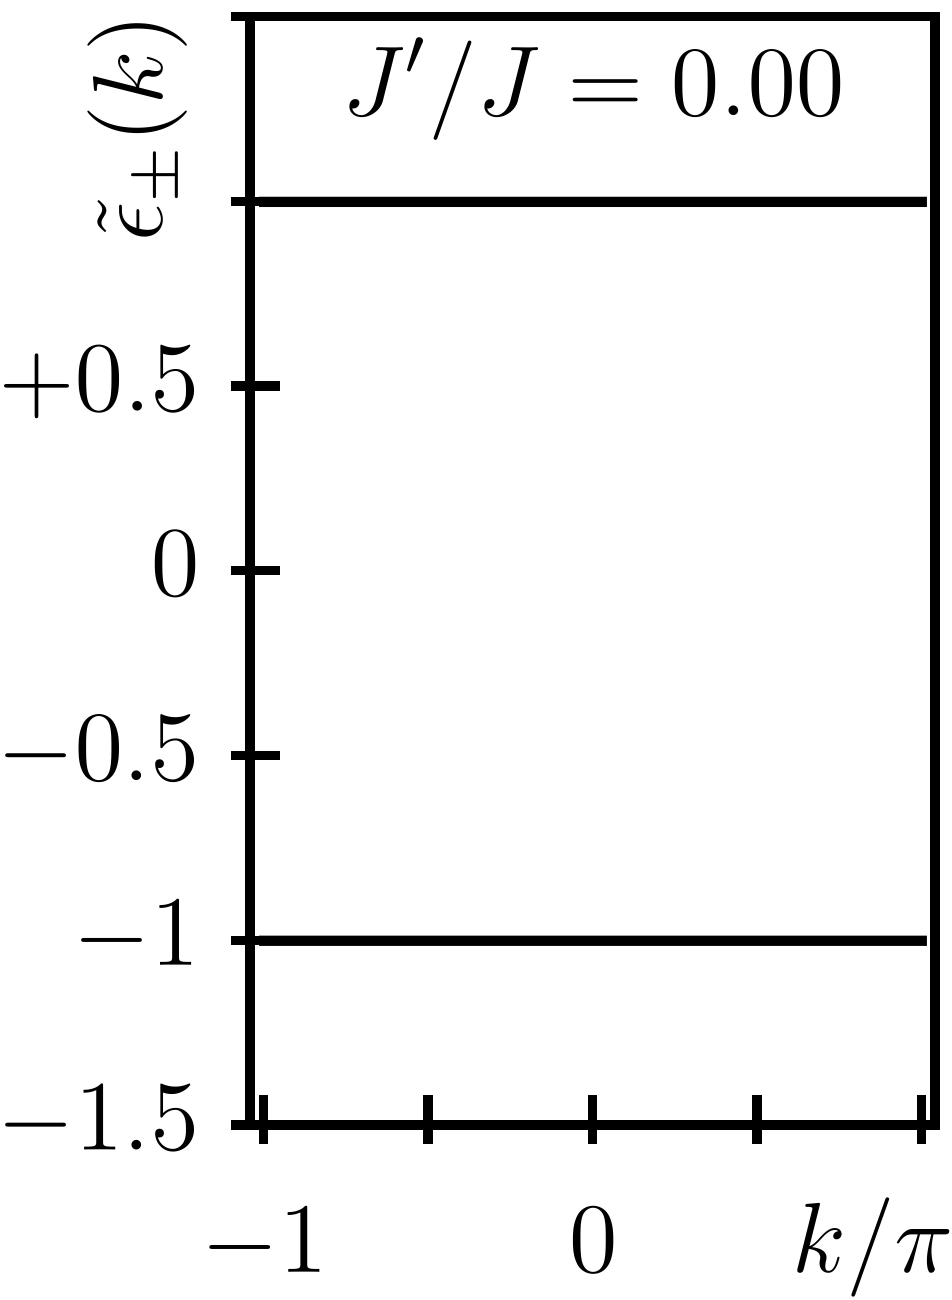
\includegraphics{figures/ssh_dispersion_0.png}
    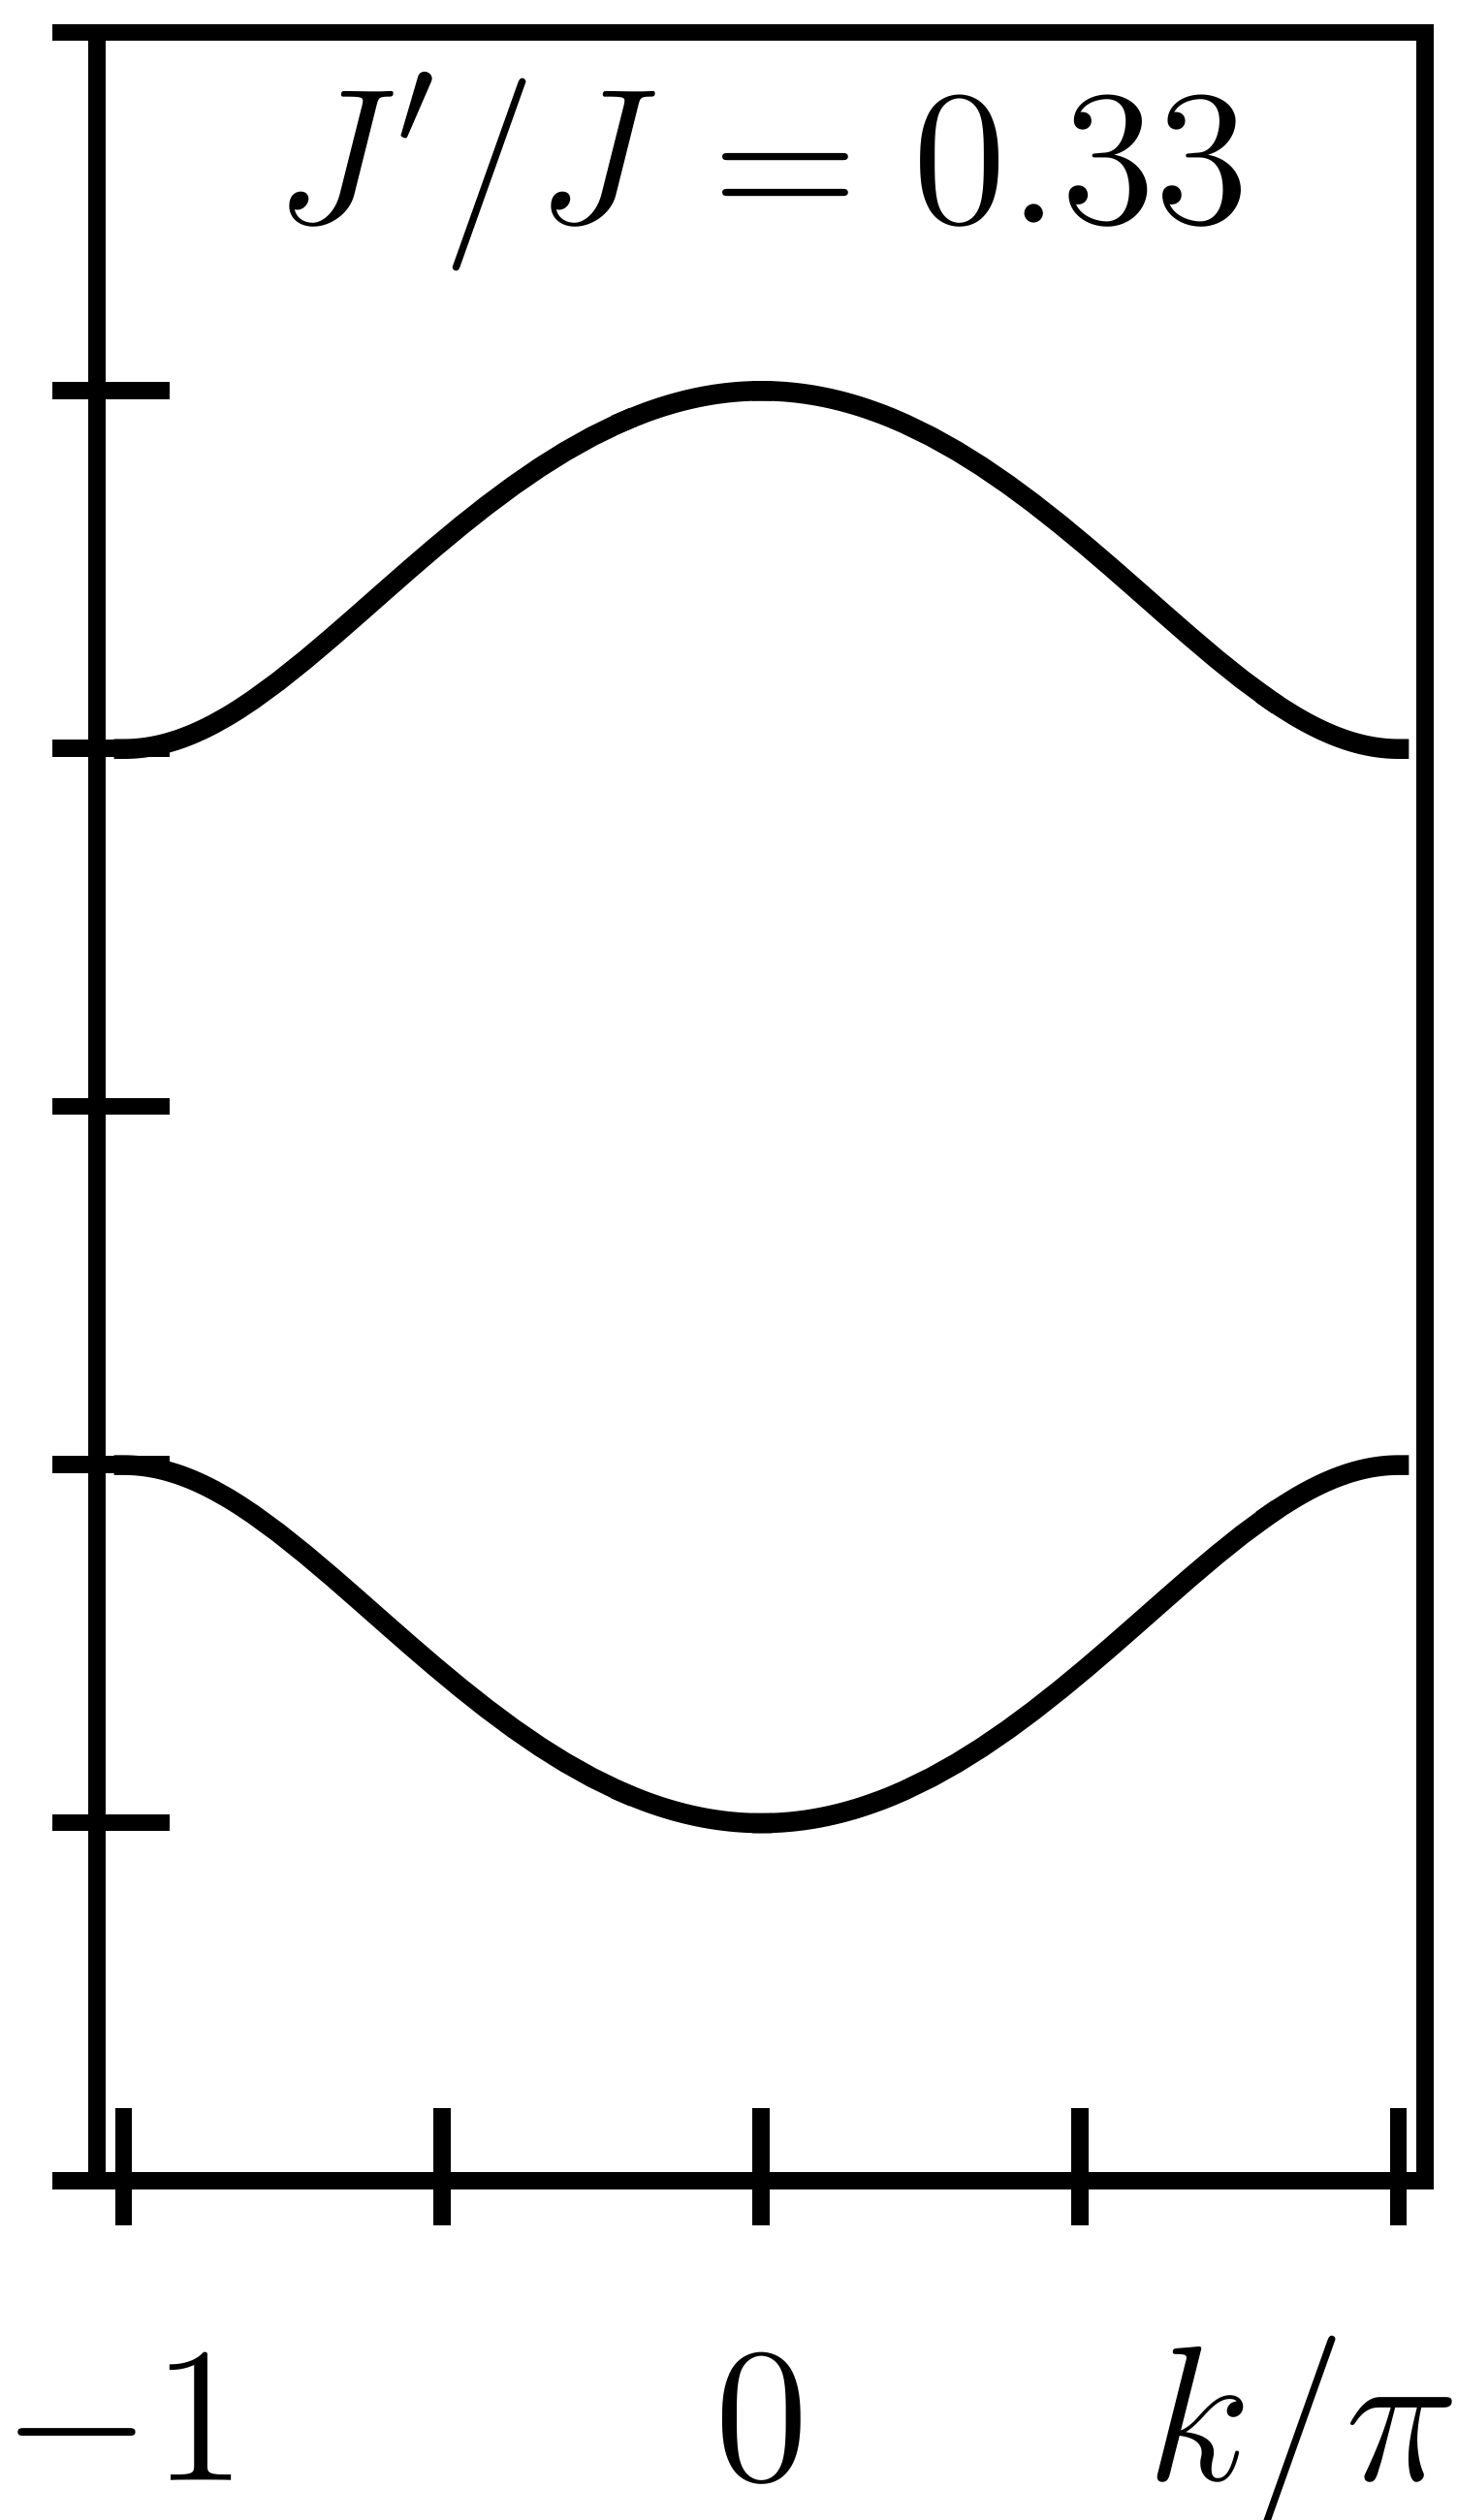
\includegraphics{figures/cropped_ssh_dispersion_1.png}
    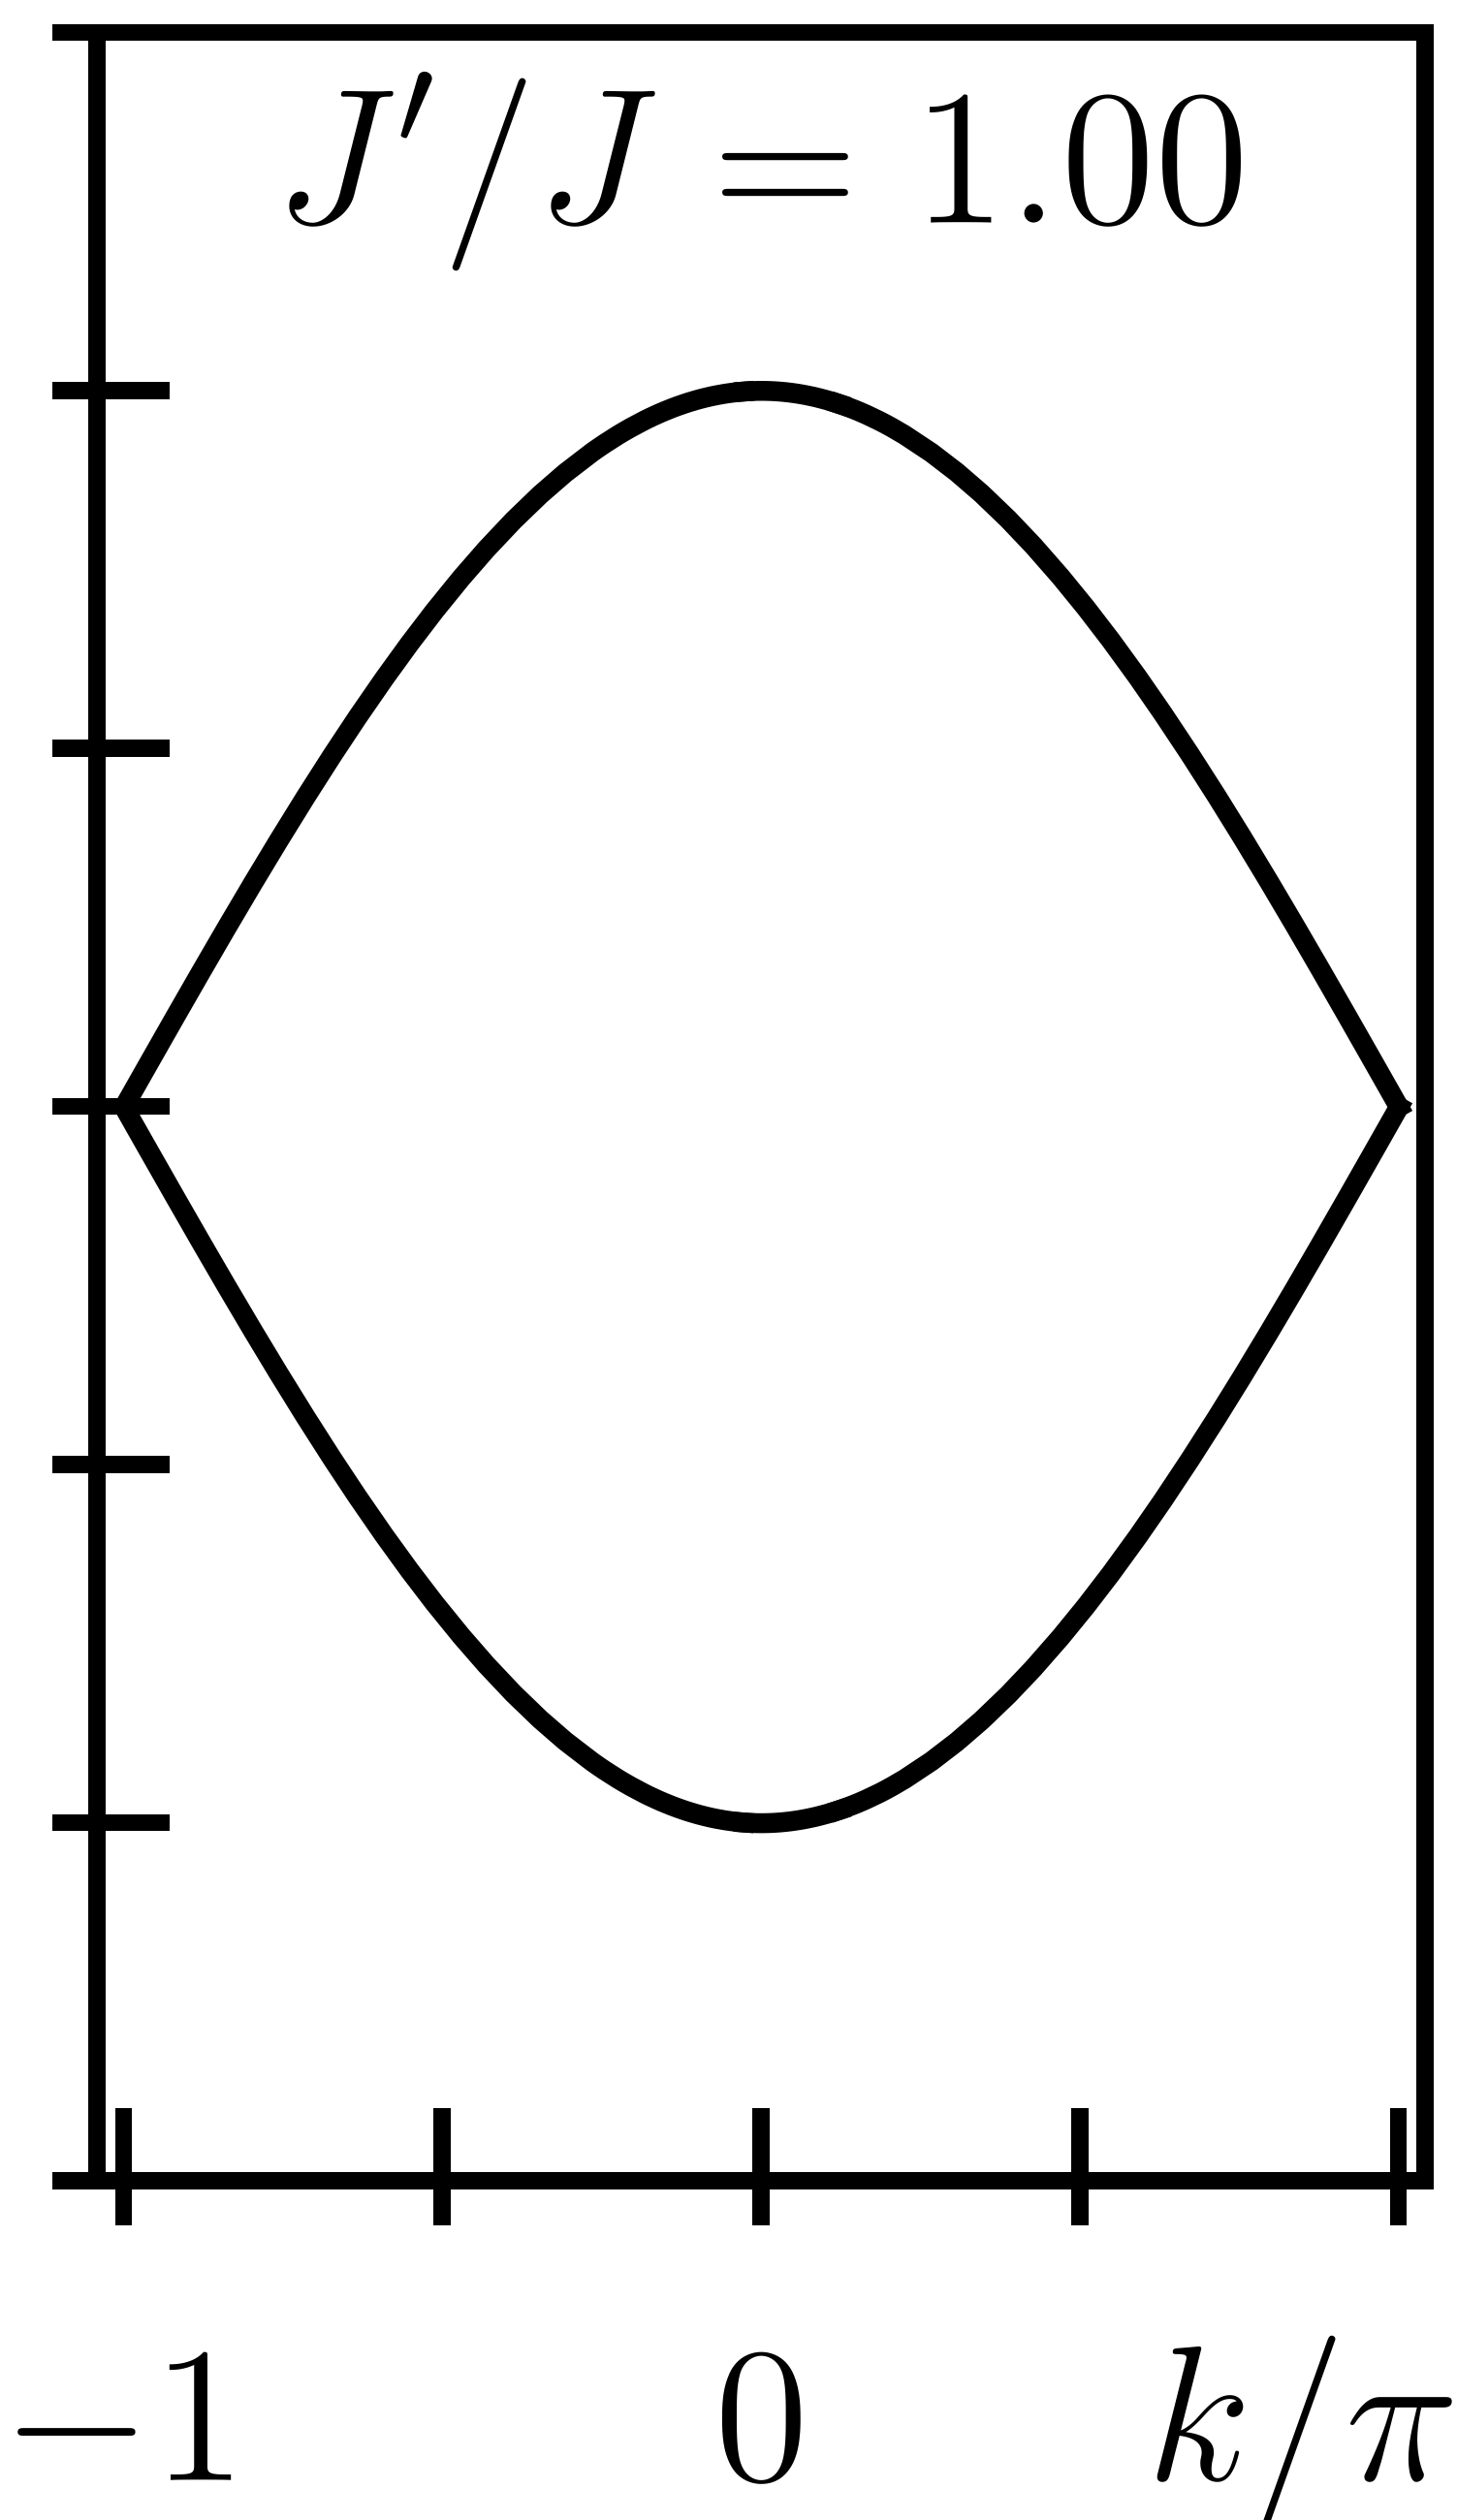
\includegraphics{figures/cropped_ssh_dispersion_2.png}
    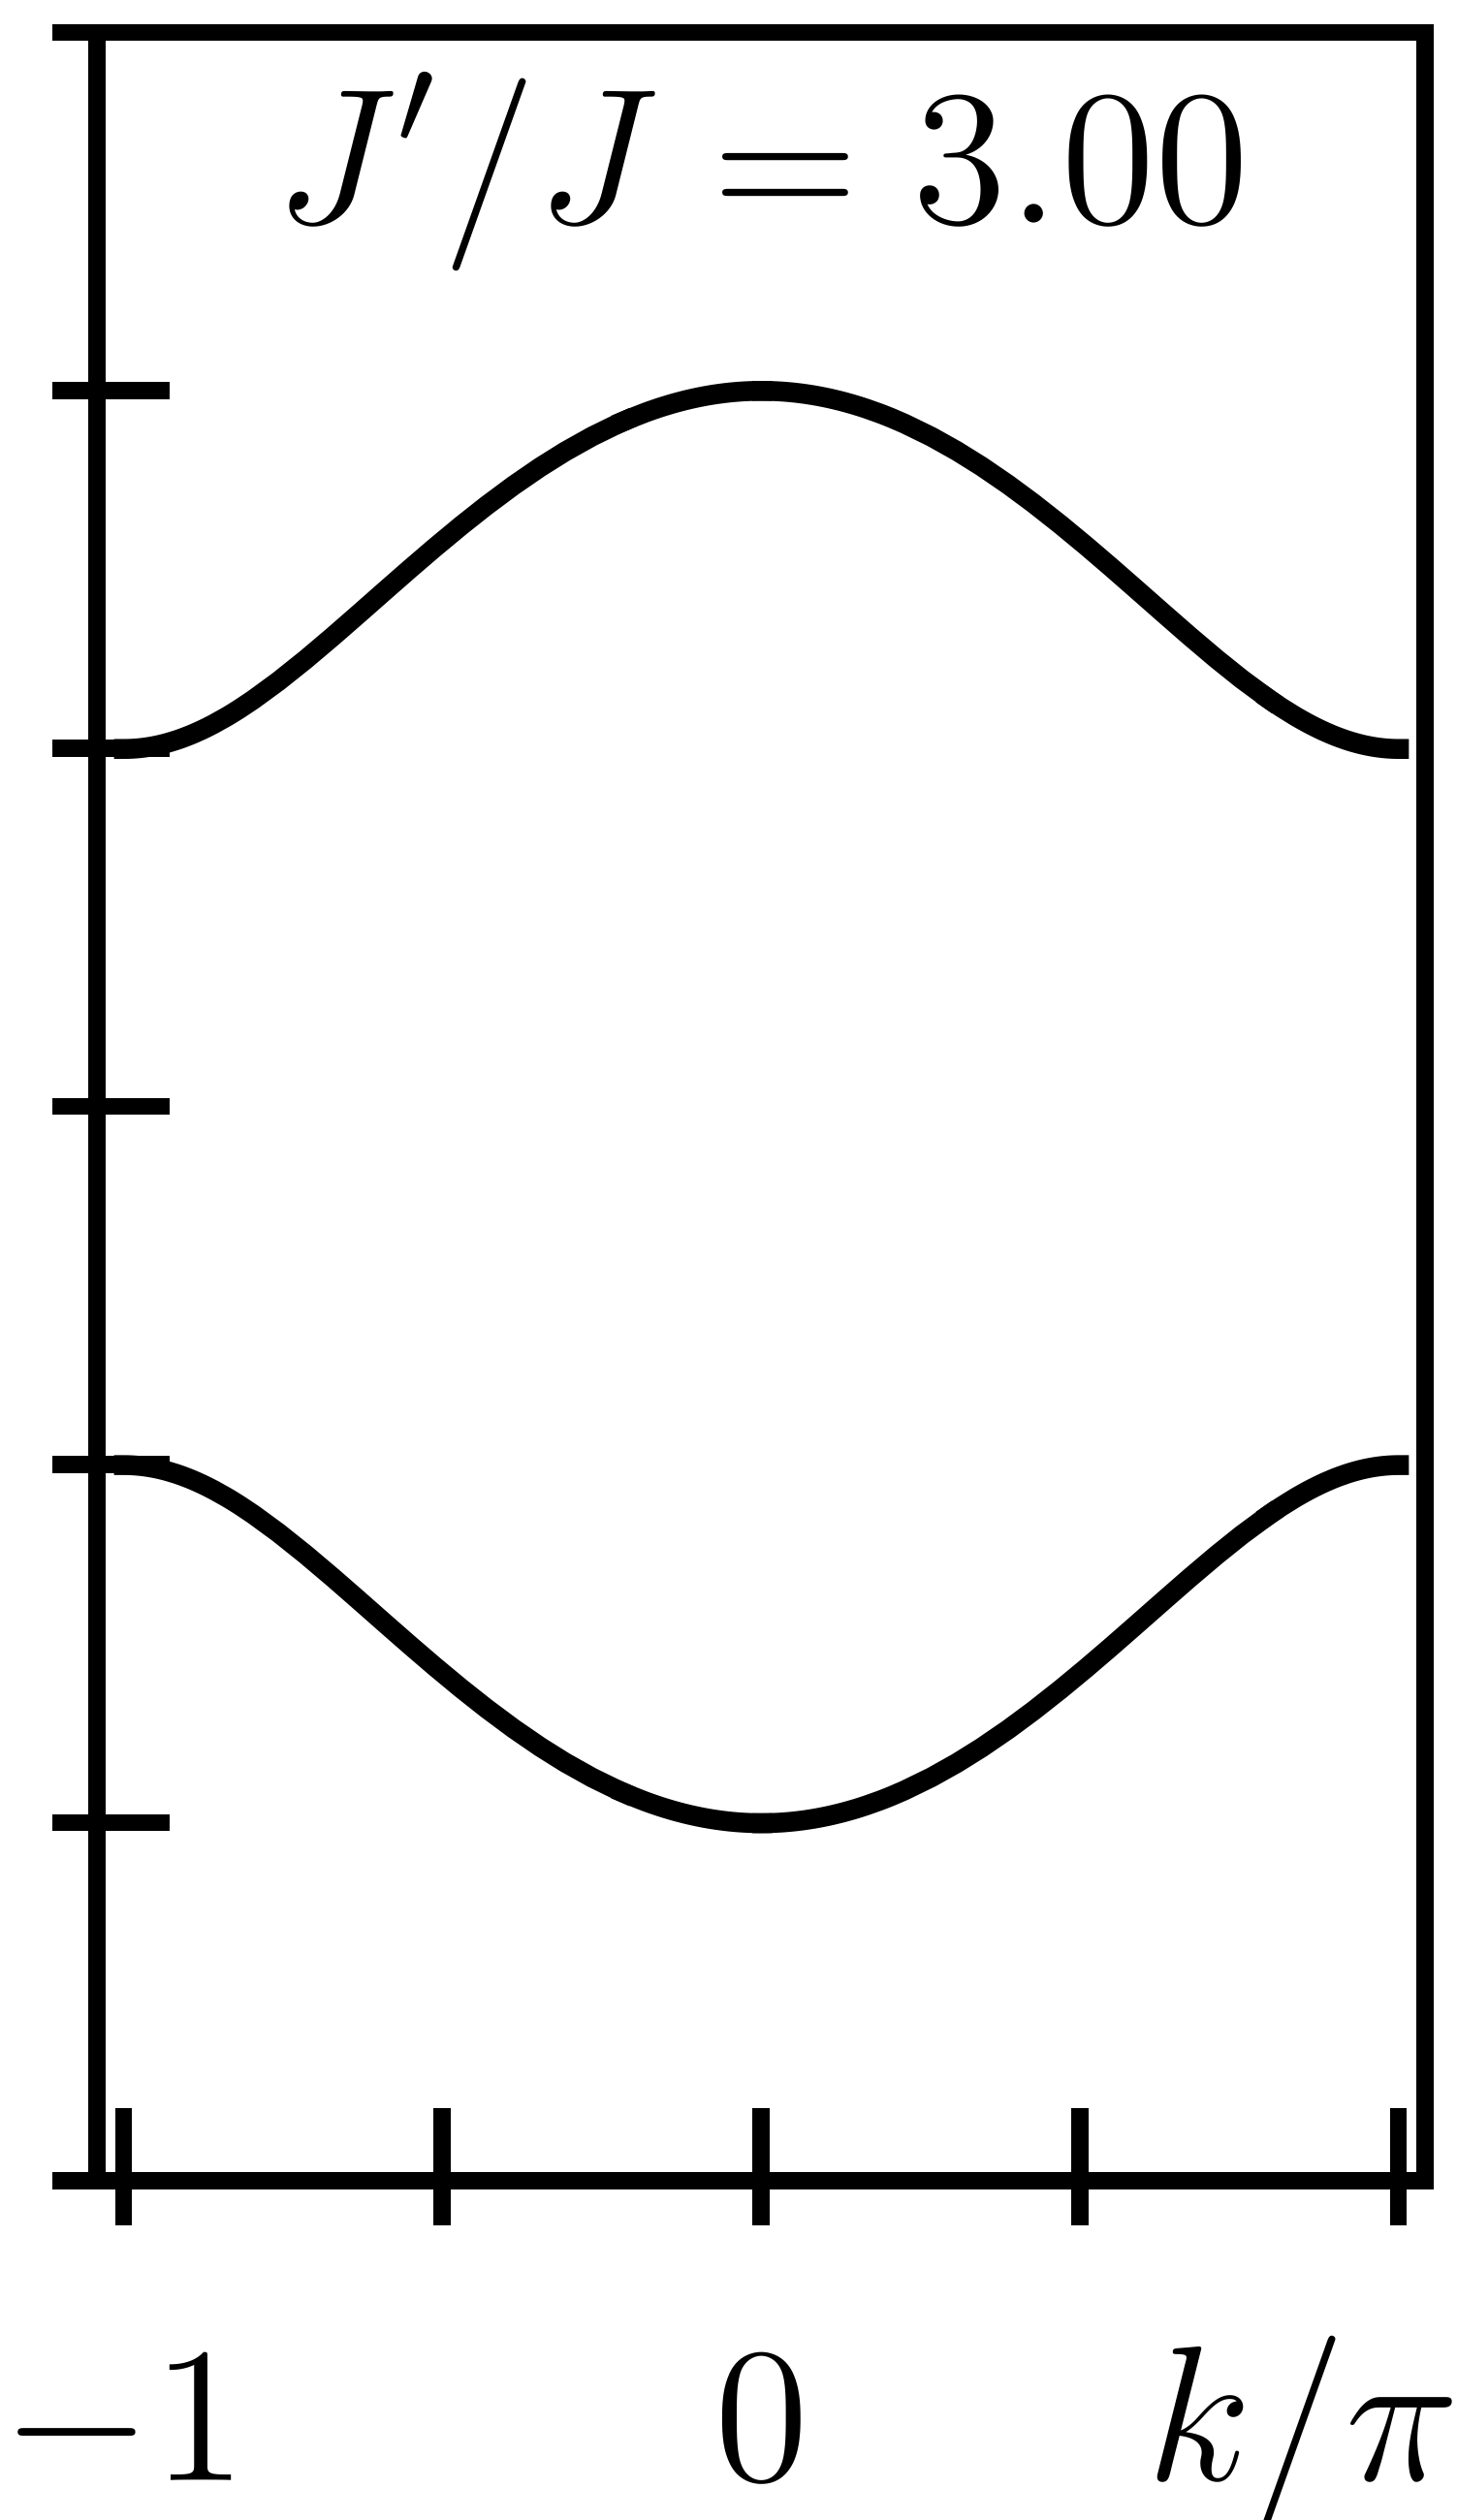
\includegraphics{figures/cropped_ssh_dispersion_3.png}
    \caption{Dimensionless band dispersion $\tilde\varepsilon_\pm(k)=\varepsilon_\pm(k)/|J+J'|$ of the SSH model for different real and positive couplings $J'/J$. The band gap $\Delta=2|J-J'|$ closes at the point $J'/J=1$ and the (dimensionless) dispersion is symmetric with respect to $J'/J\rightarrow J/J'$.}
    \label{fig:ssh_dispersion}
\end{figure}

Let us explore more the topological equivalency we detailed in the previous section.
The valence/conduction band shows a maximum/minimum at $k=\pi$, resulting in a band gap of size $\Delta = 2\left|J-J'\right|$.
As long as $J\neq J'$, the band gap $\Delta\neq0$ is preserved, and for reasons explained shortly, we call $J>J'$ trivial insulator (TRI) and $J<J'$ topological insulator (TOI).
Within each of those phases, all Hamiltonians are topologically equivalent.
It is also possible to define a family of Hamiltonians according to
\begin{align}
    H(t,k) =
    \begin{pmatrix}
        \sin(\pi t) & 1-t + t\re^{-\ri k} \\
        1-t + t\re^{\ri k} & -\sin(\pi t)
    \end{pmatrix},
    \label{eq:hamiltonian_path}
\end{align}
which is equivalent to the Bloch vector
\begin{align}
    B_x(t,k) = (1-t)+t\cos(k),
    \quad
    B_y(t,k) = t\sin(k),
    \quad
    B_z(t,k) = \sin(\pi t).
\end{align}
\begin{figure}[ht]
    \centering
    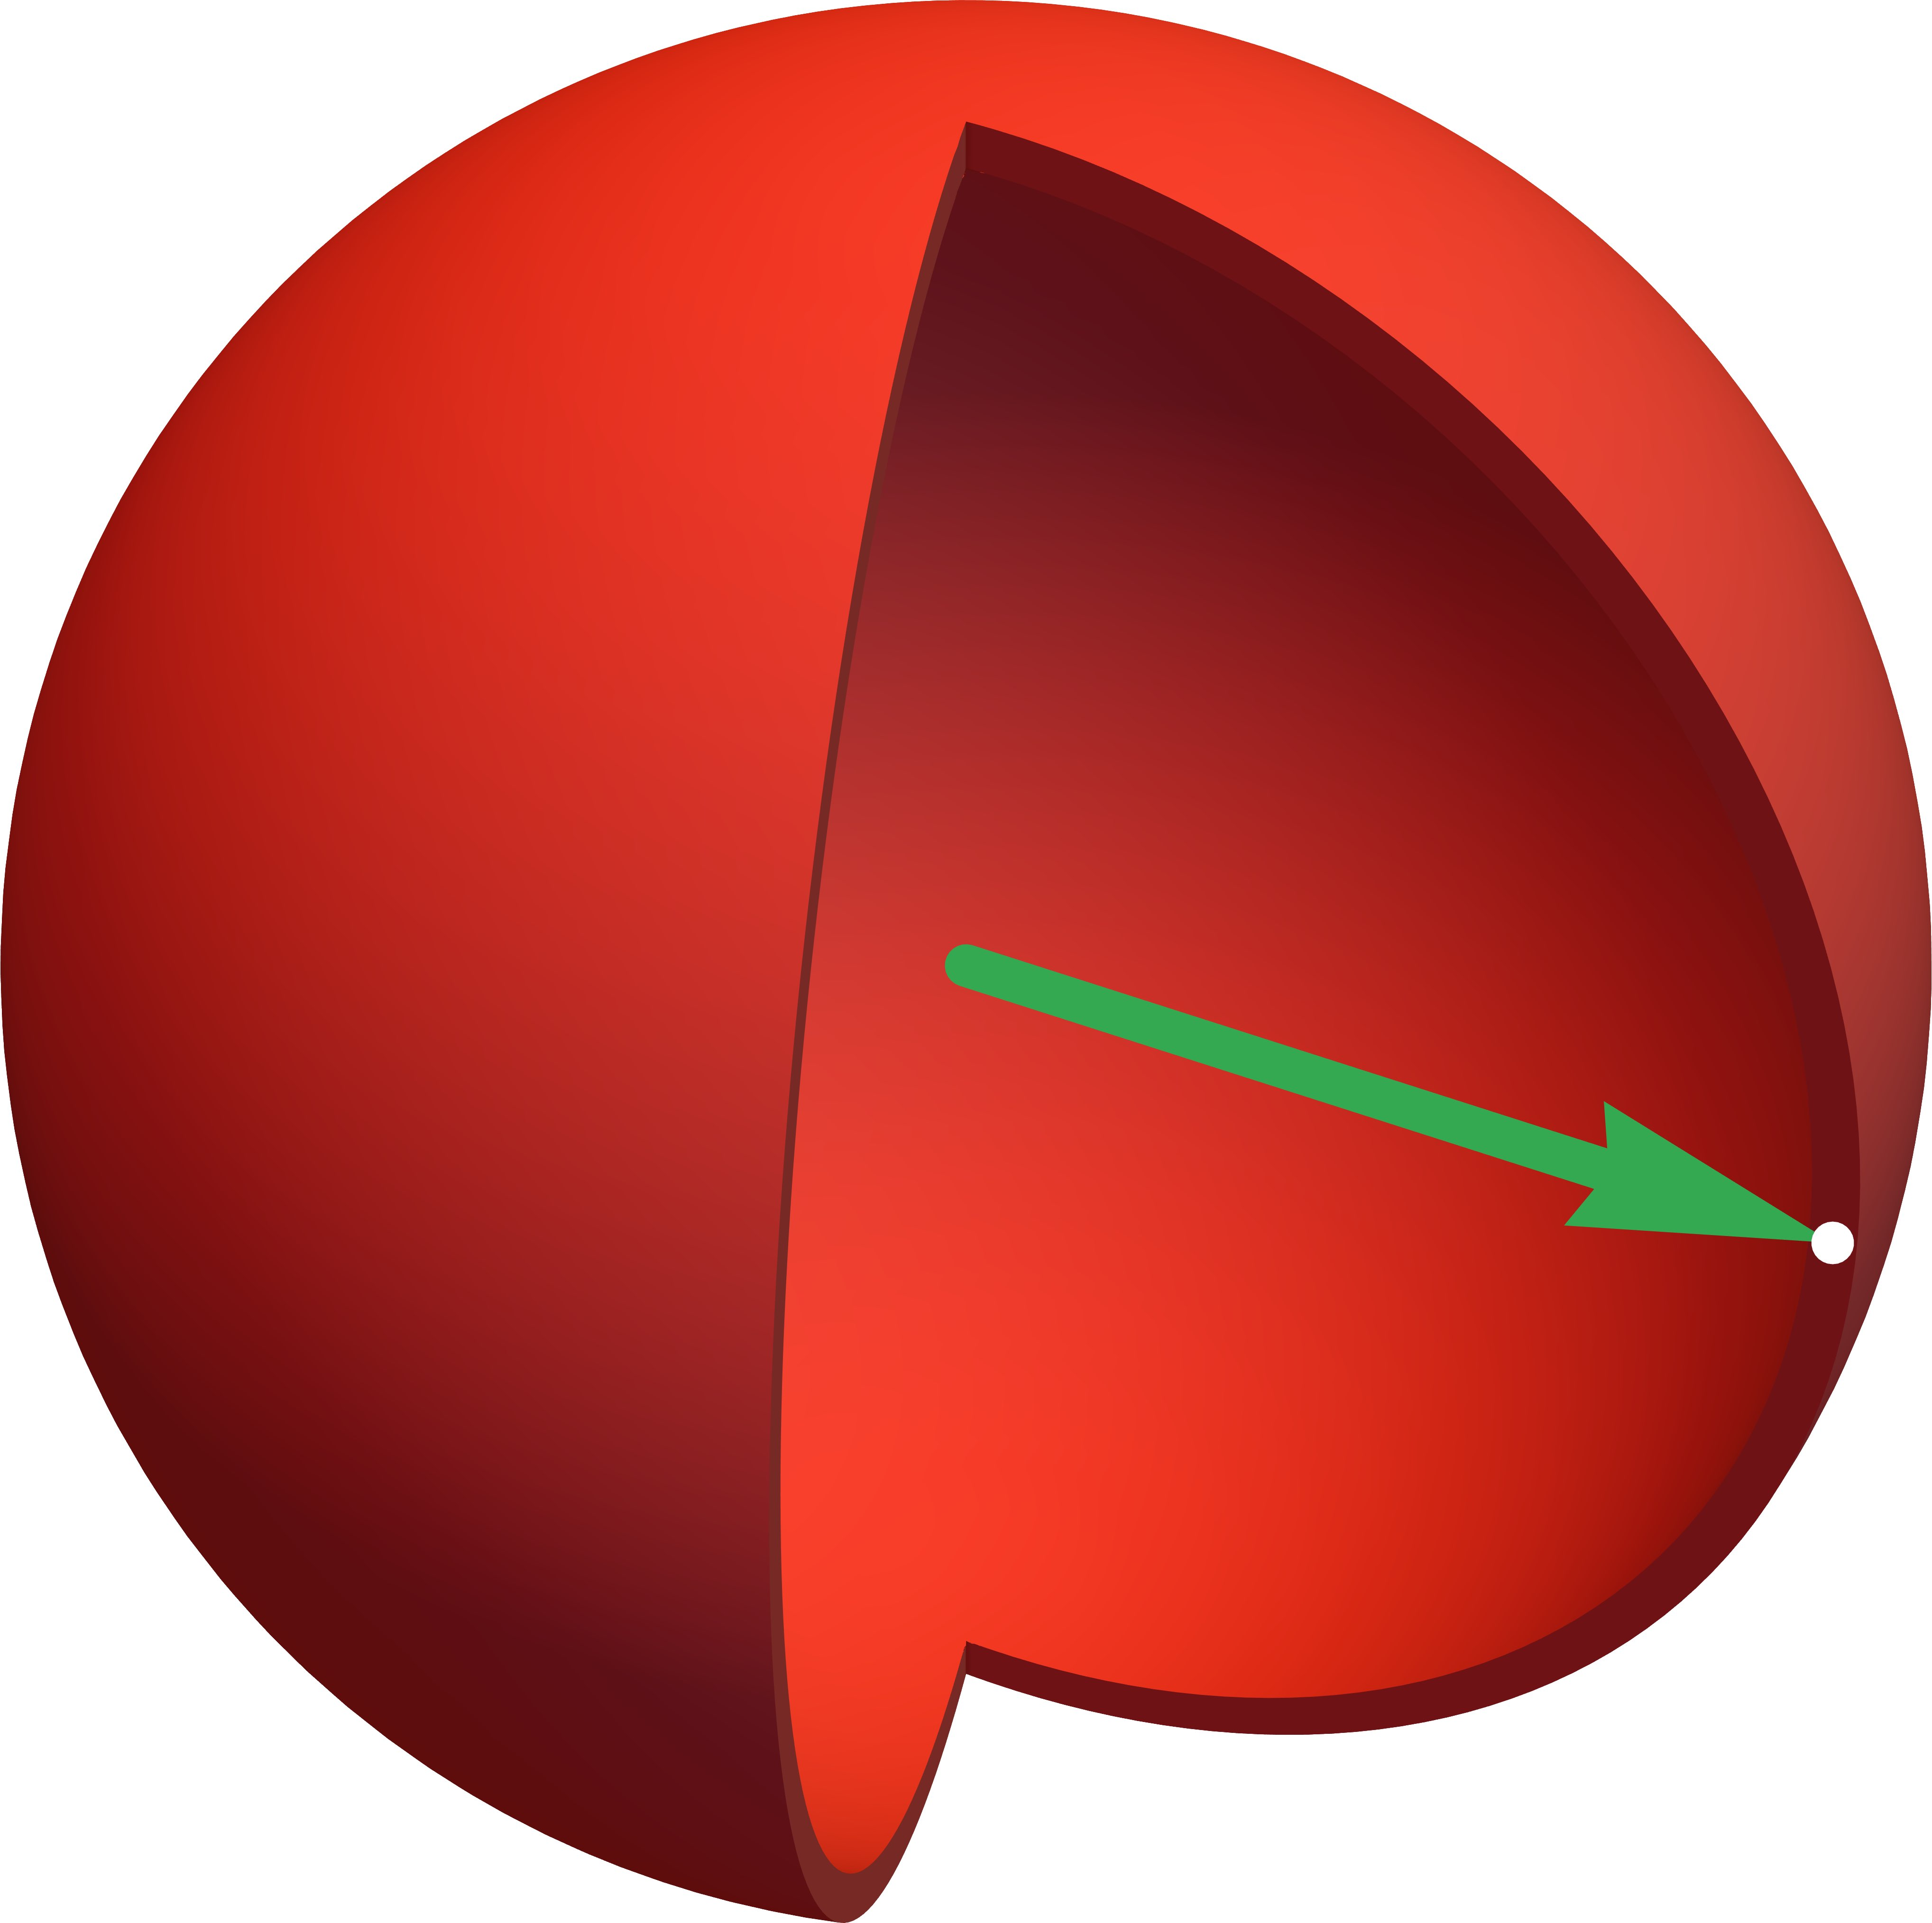
\includegraphics[width=0.13\textwidth]{figures/ssh_deformed_normalized_bloch_vector_t0_000.jpg}
    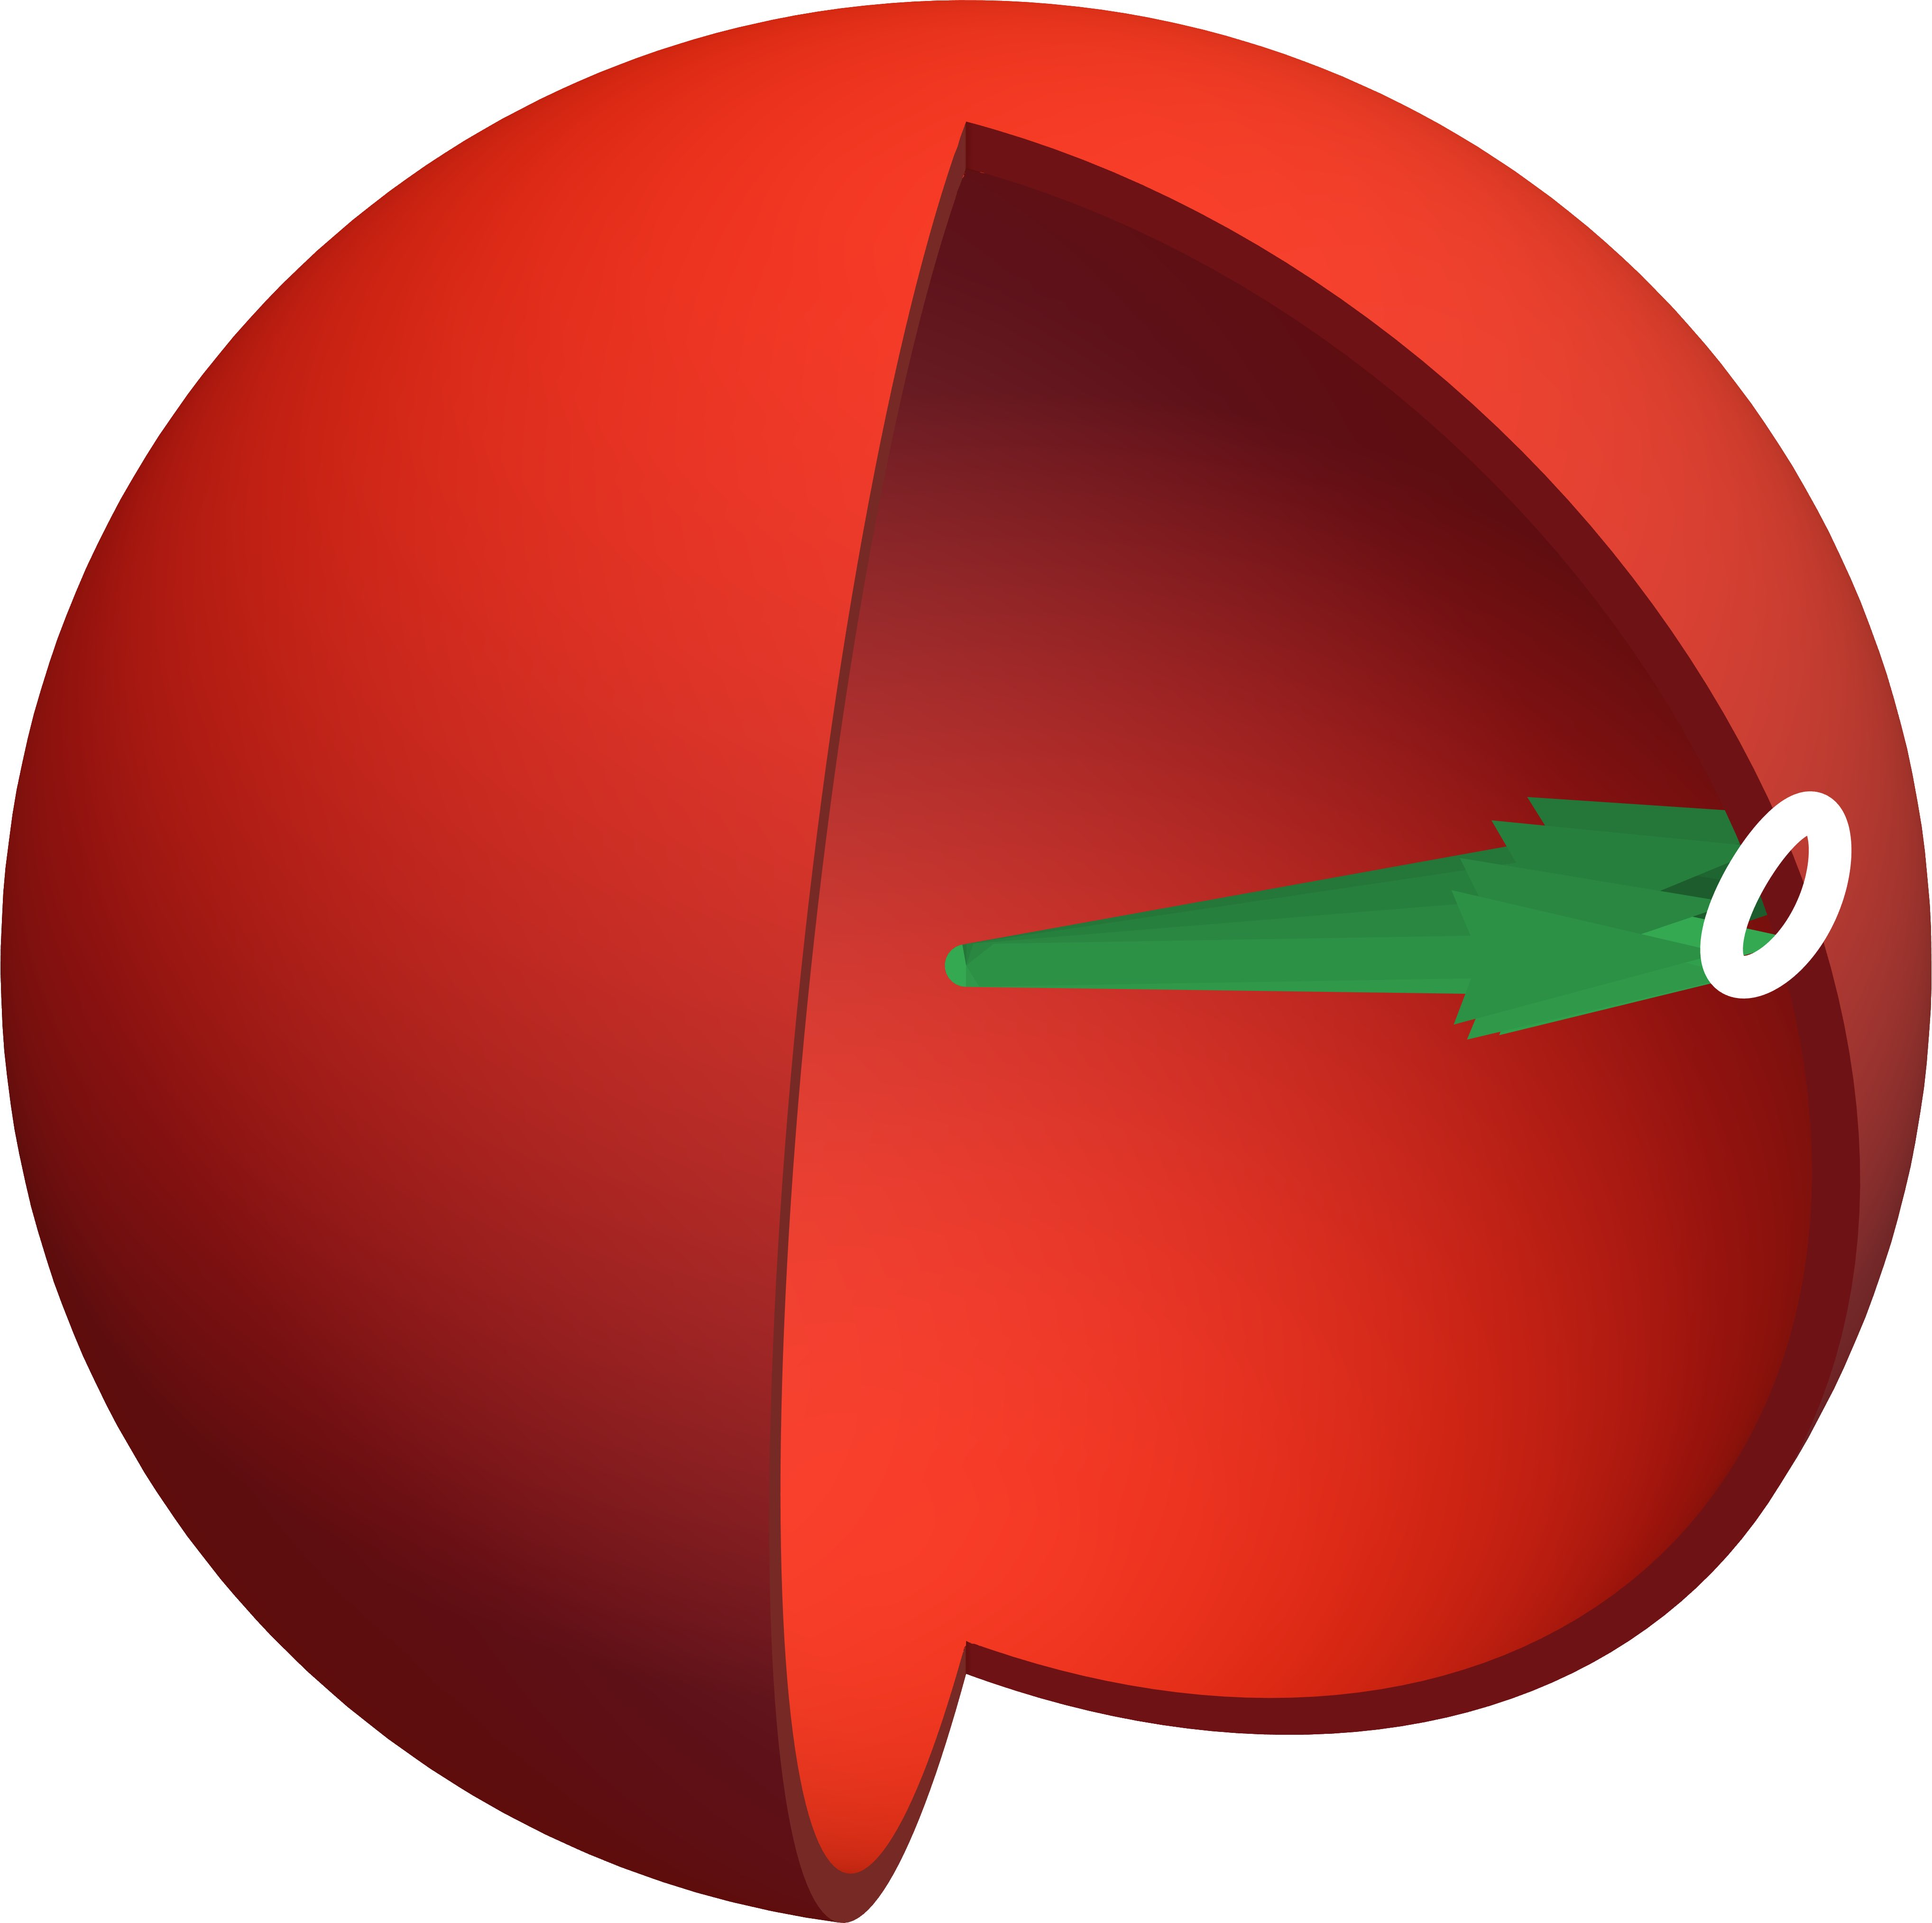
\includegraphics[width=0.13\textwidth]{figures/ssh_deformed_normalized_bloch_vector_t0_125.jpg}
    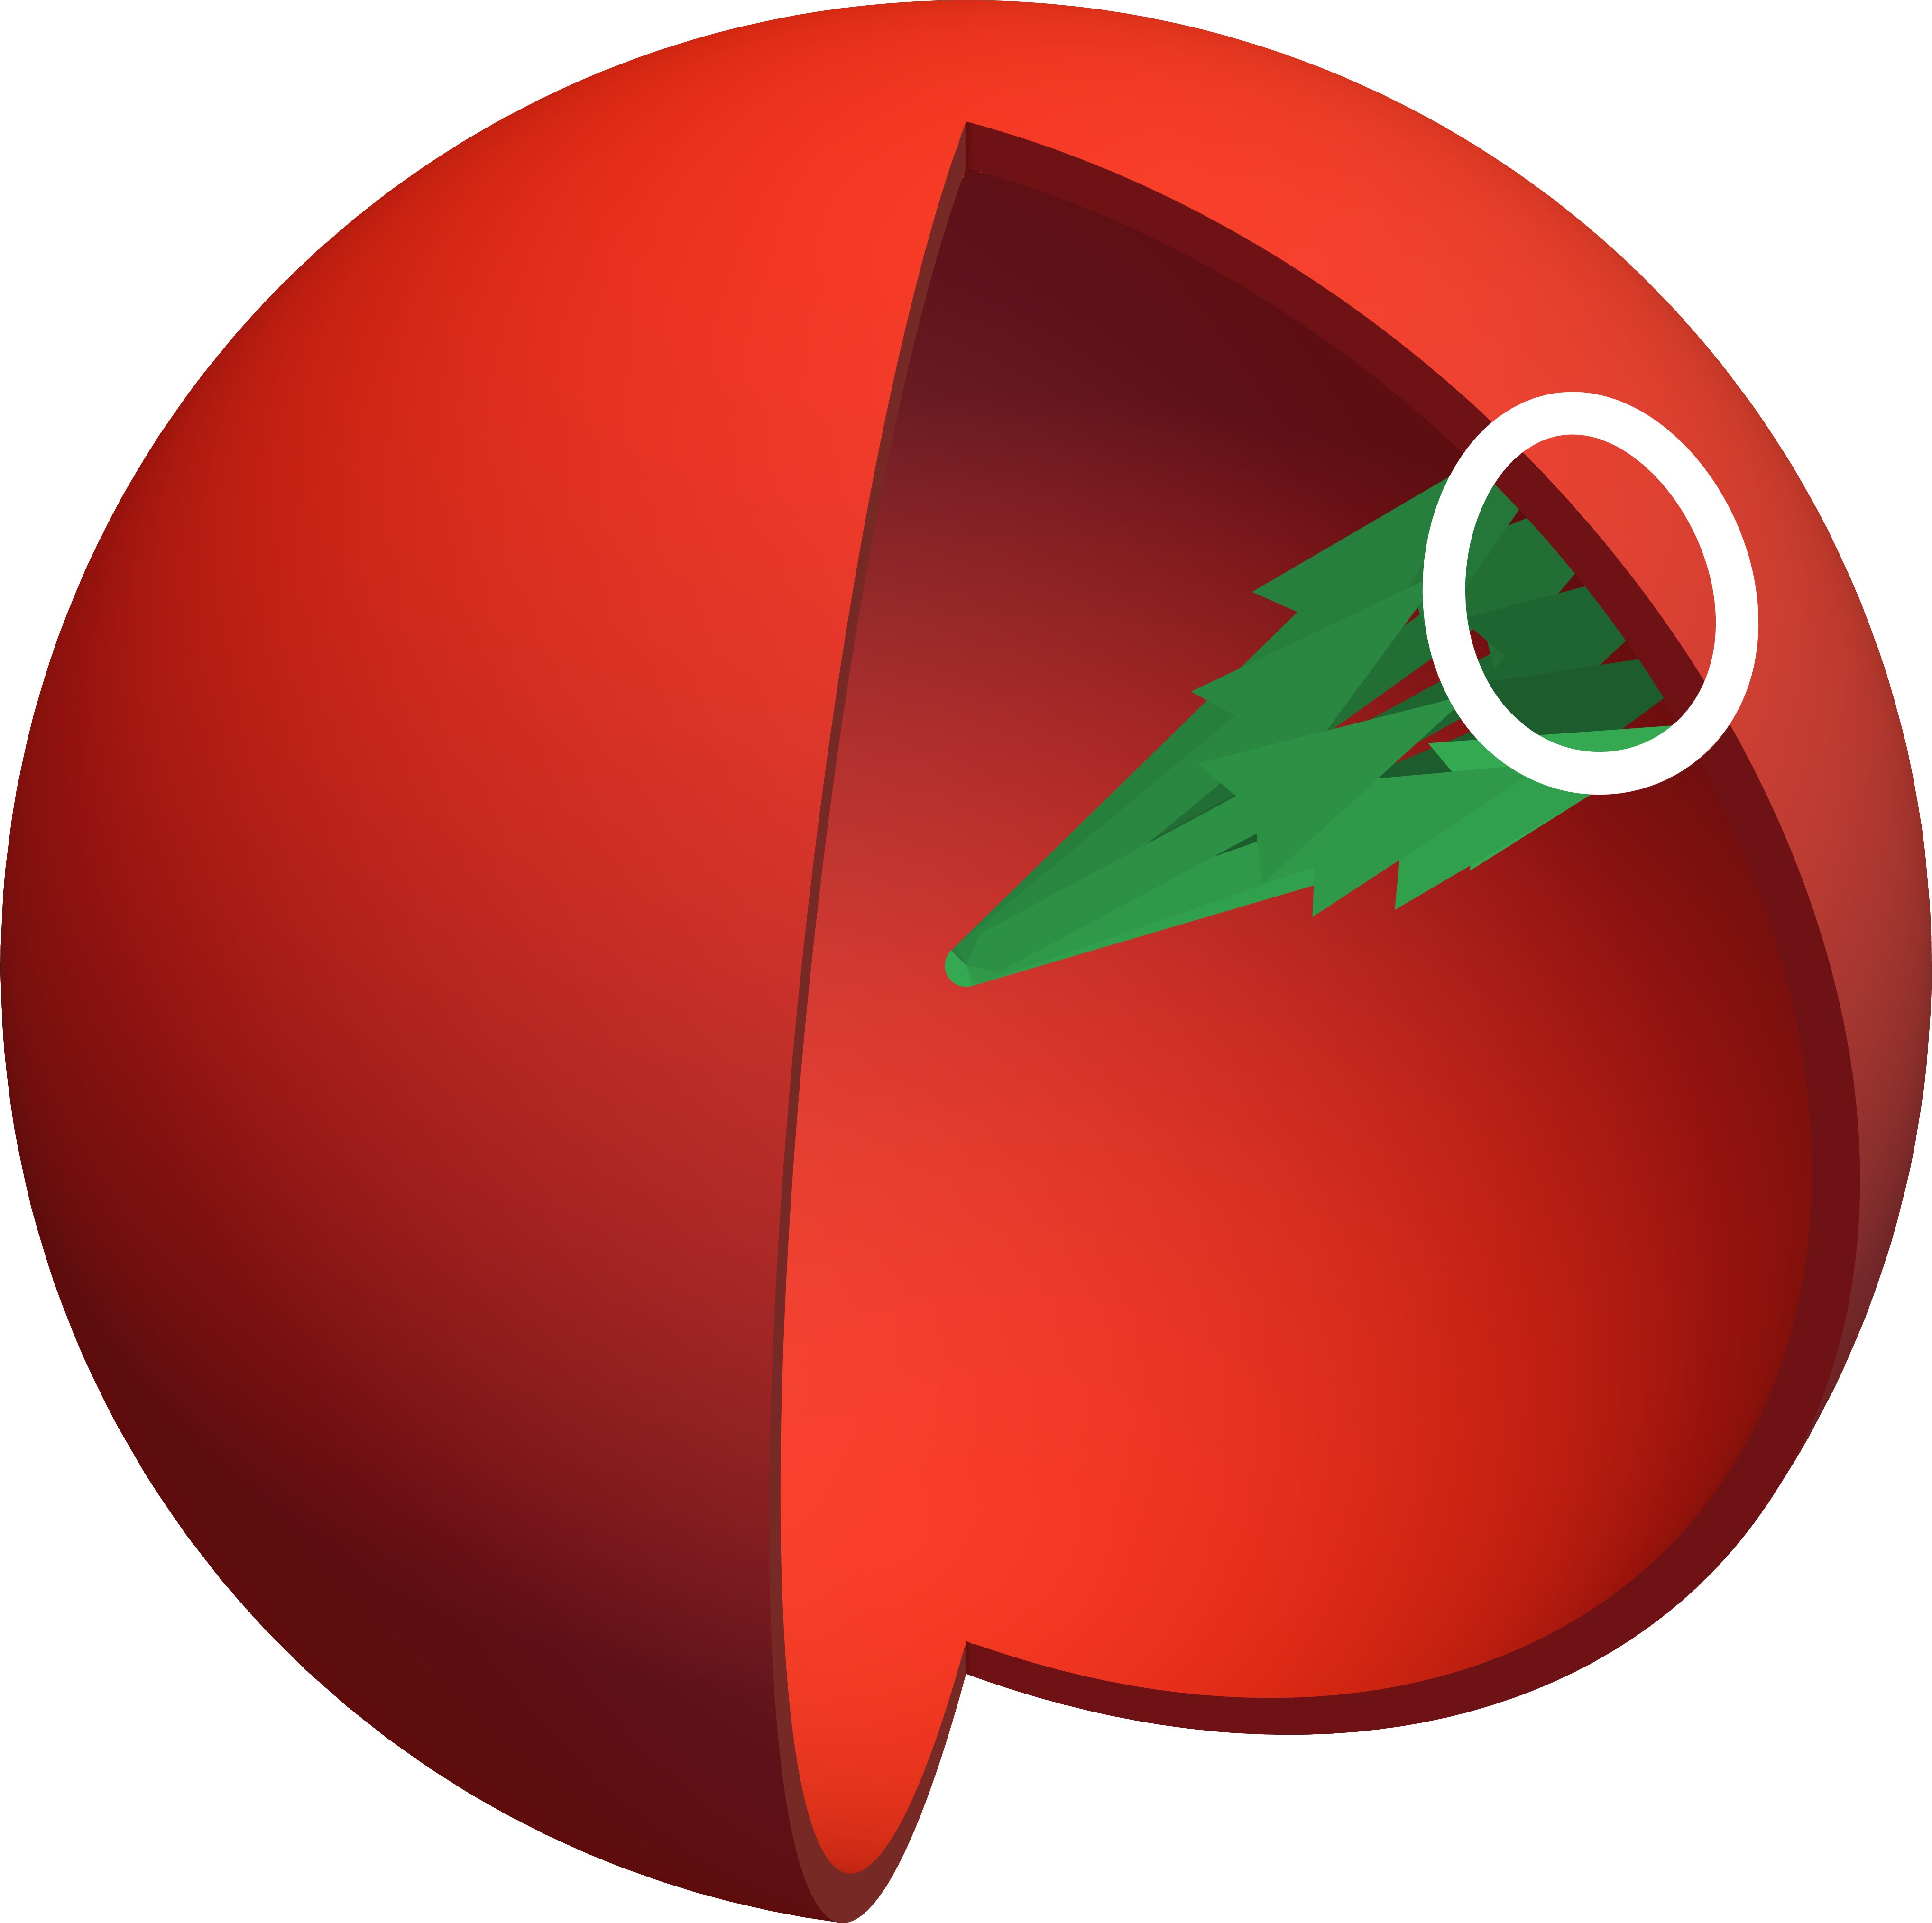
\includegraphics[width=0.13\textwidth]{figures/ssh_deformed_normalized_bloch_vector_t0_250.jpg}
    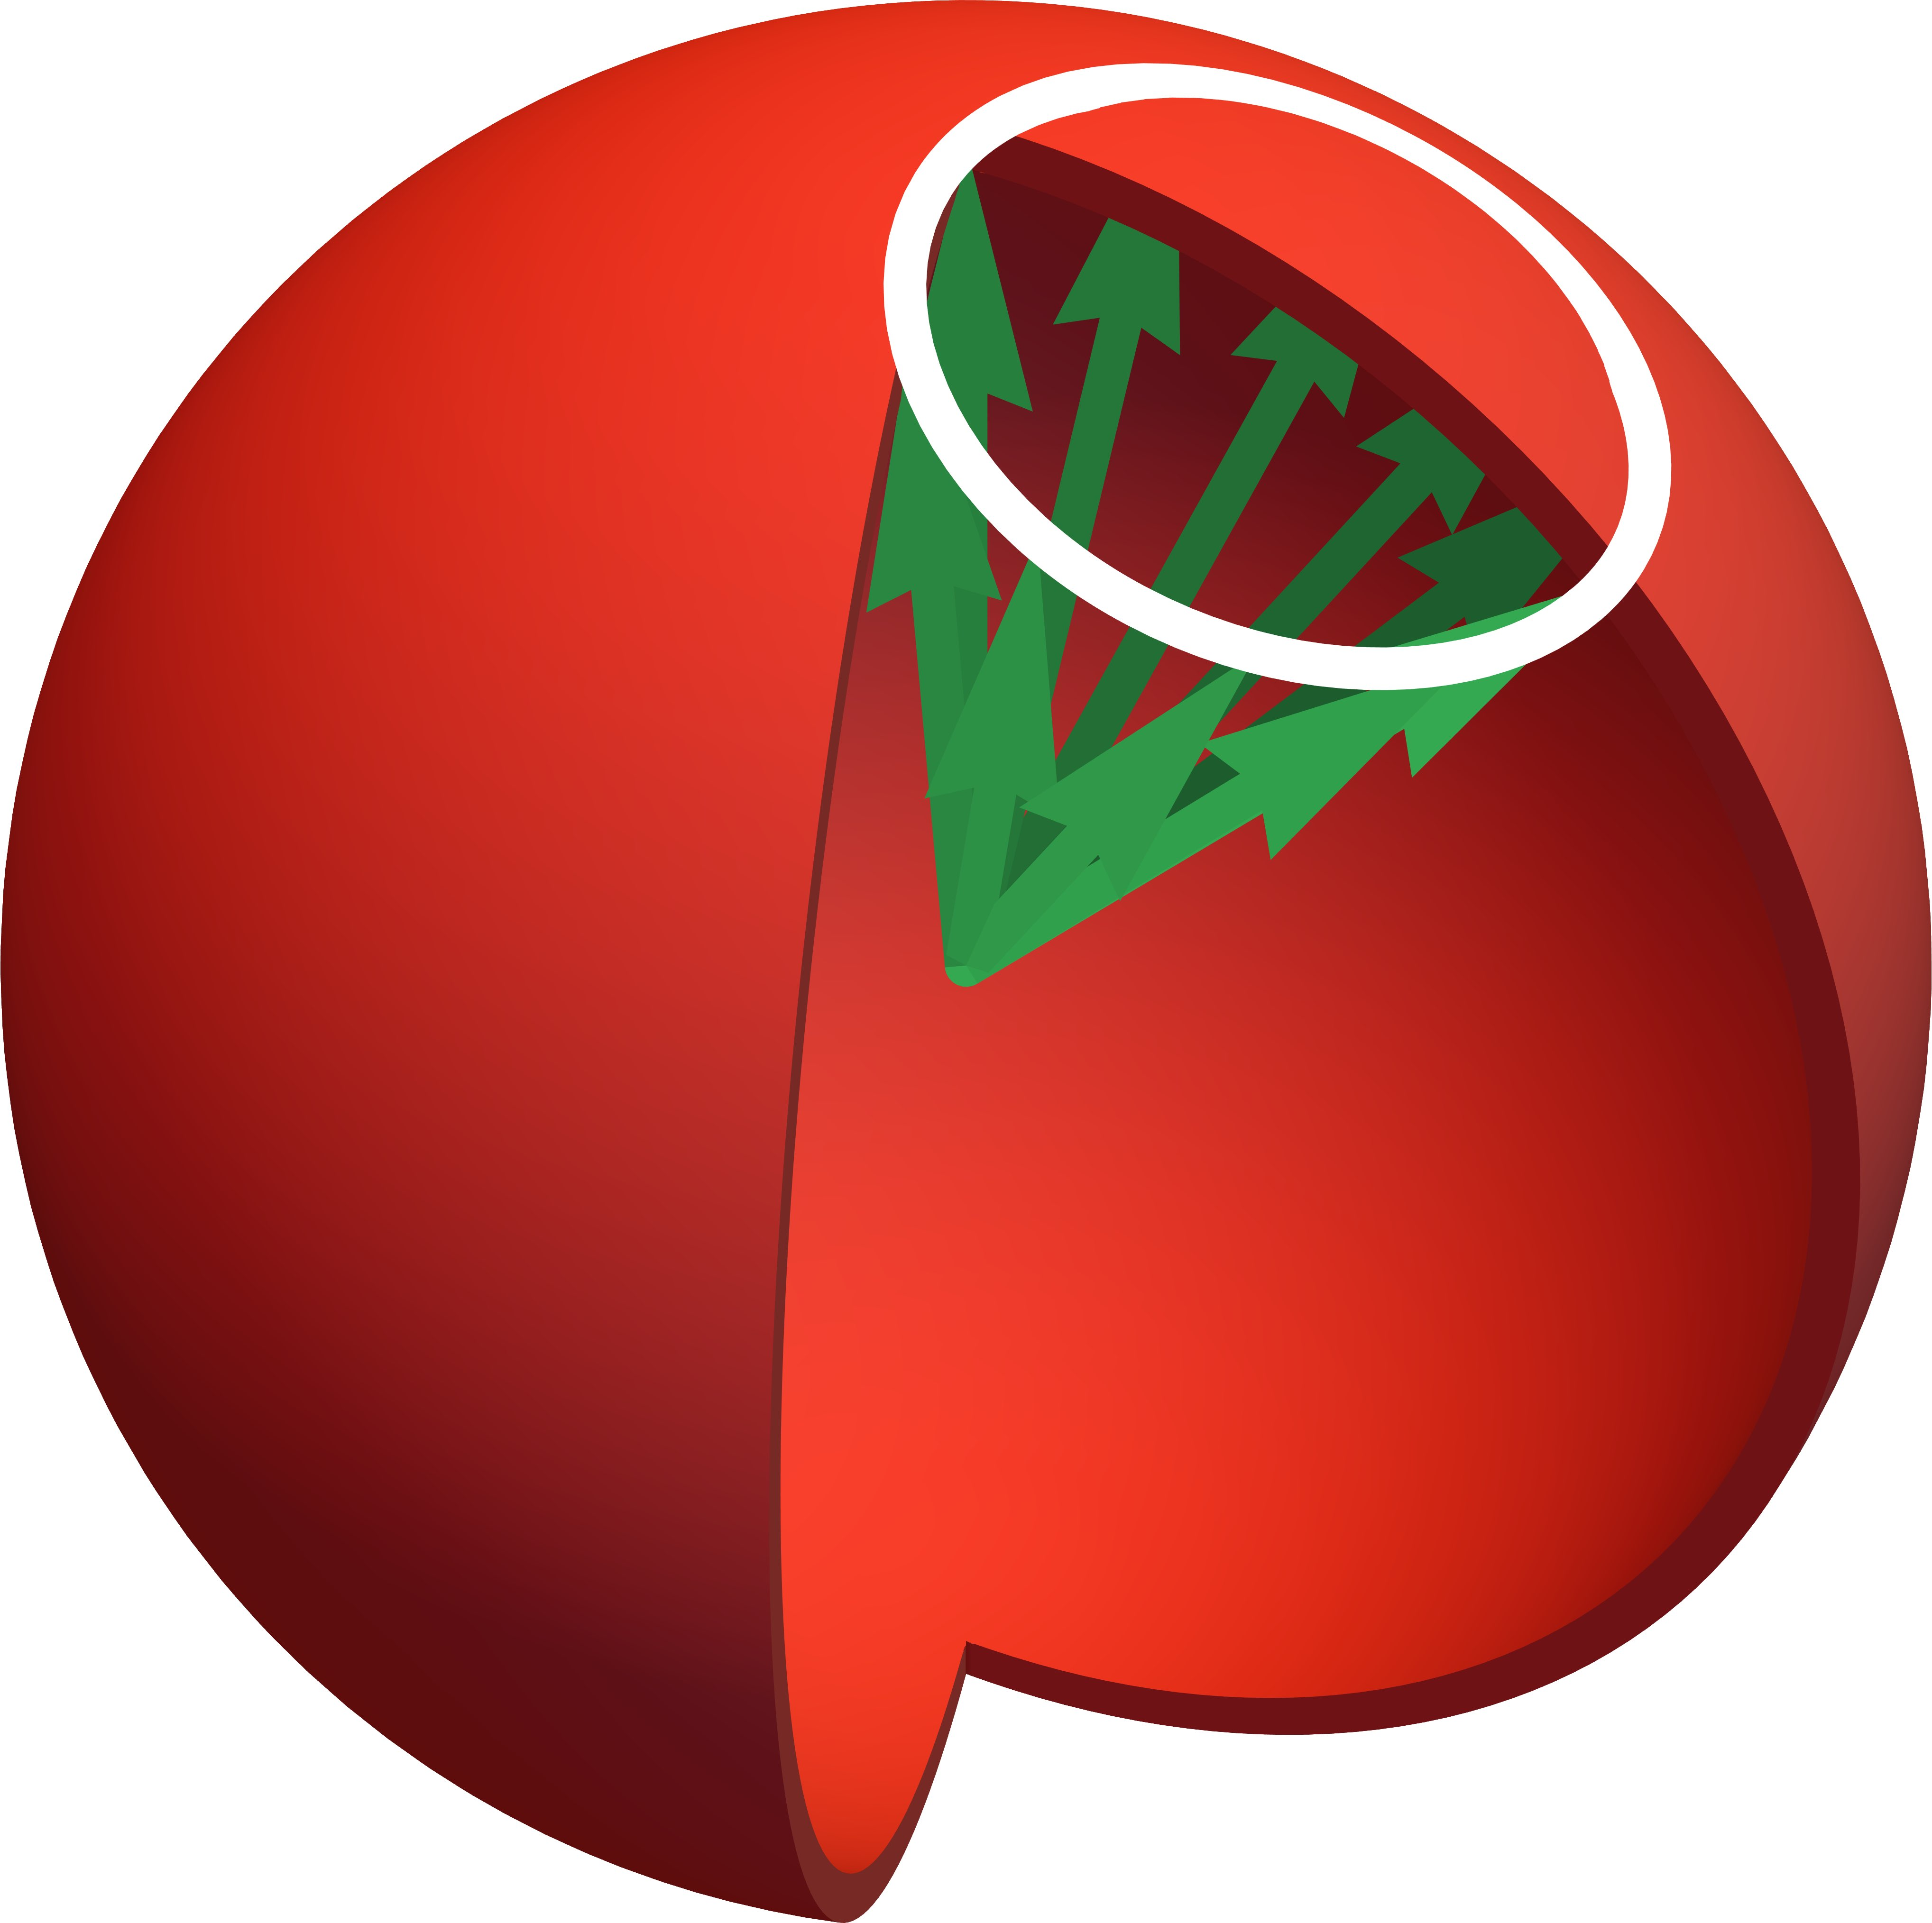
\includegraphics[width=0.13\textwidth]{figures/ssh_deformed_normalized_bloch_vector_t0_500.jpg}
    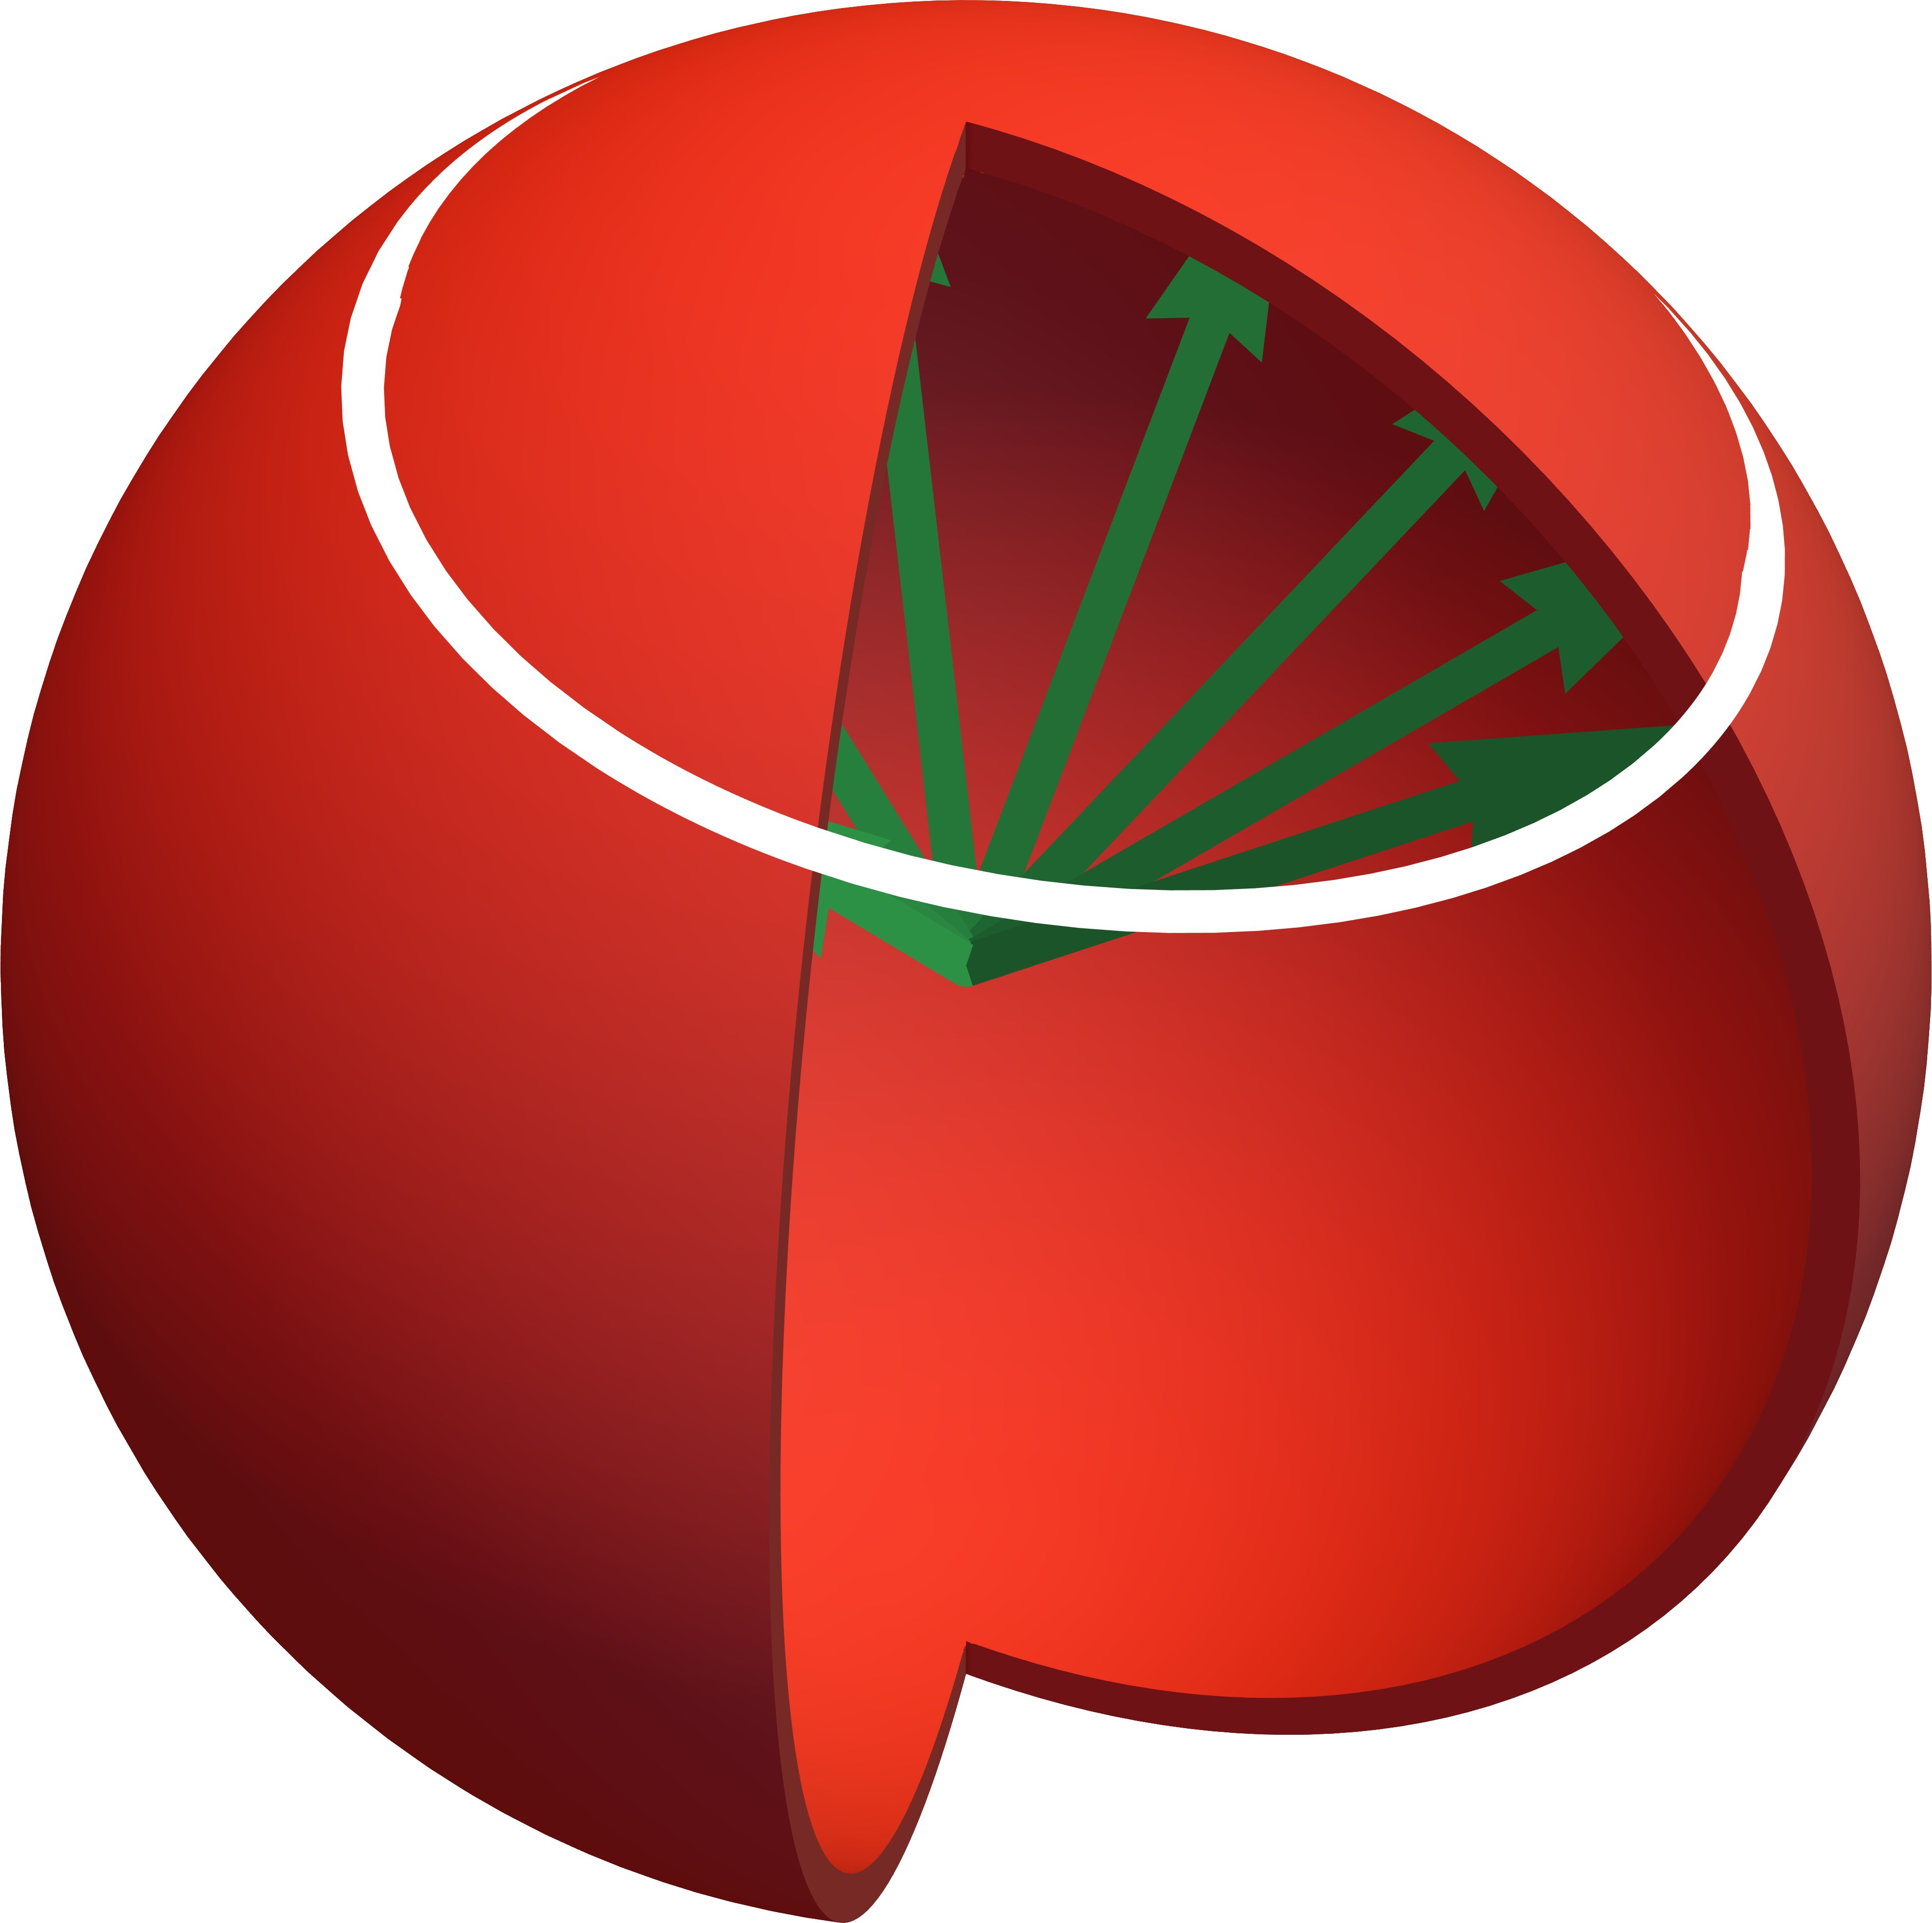
\includegraphics[width=0.13\textwidth]{figures/ssh_deformed_normalized_bloch_vector_t0_750.jpg}
    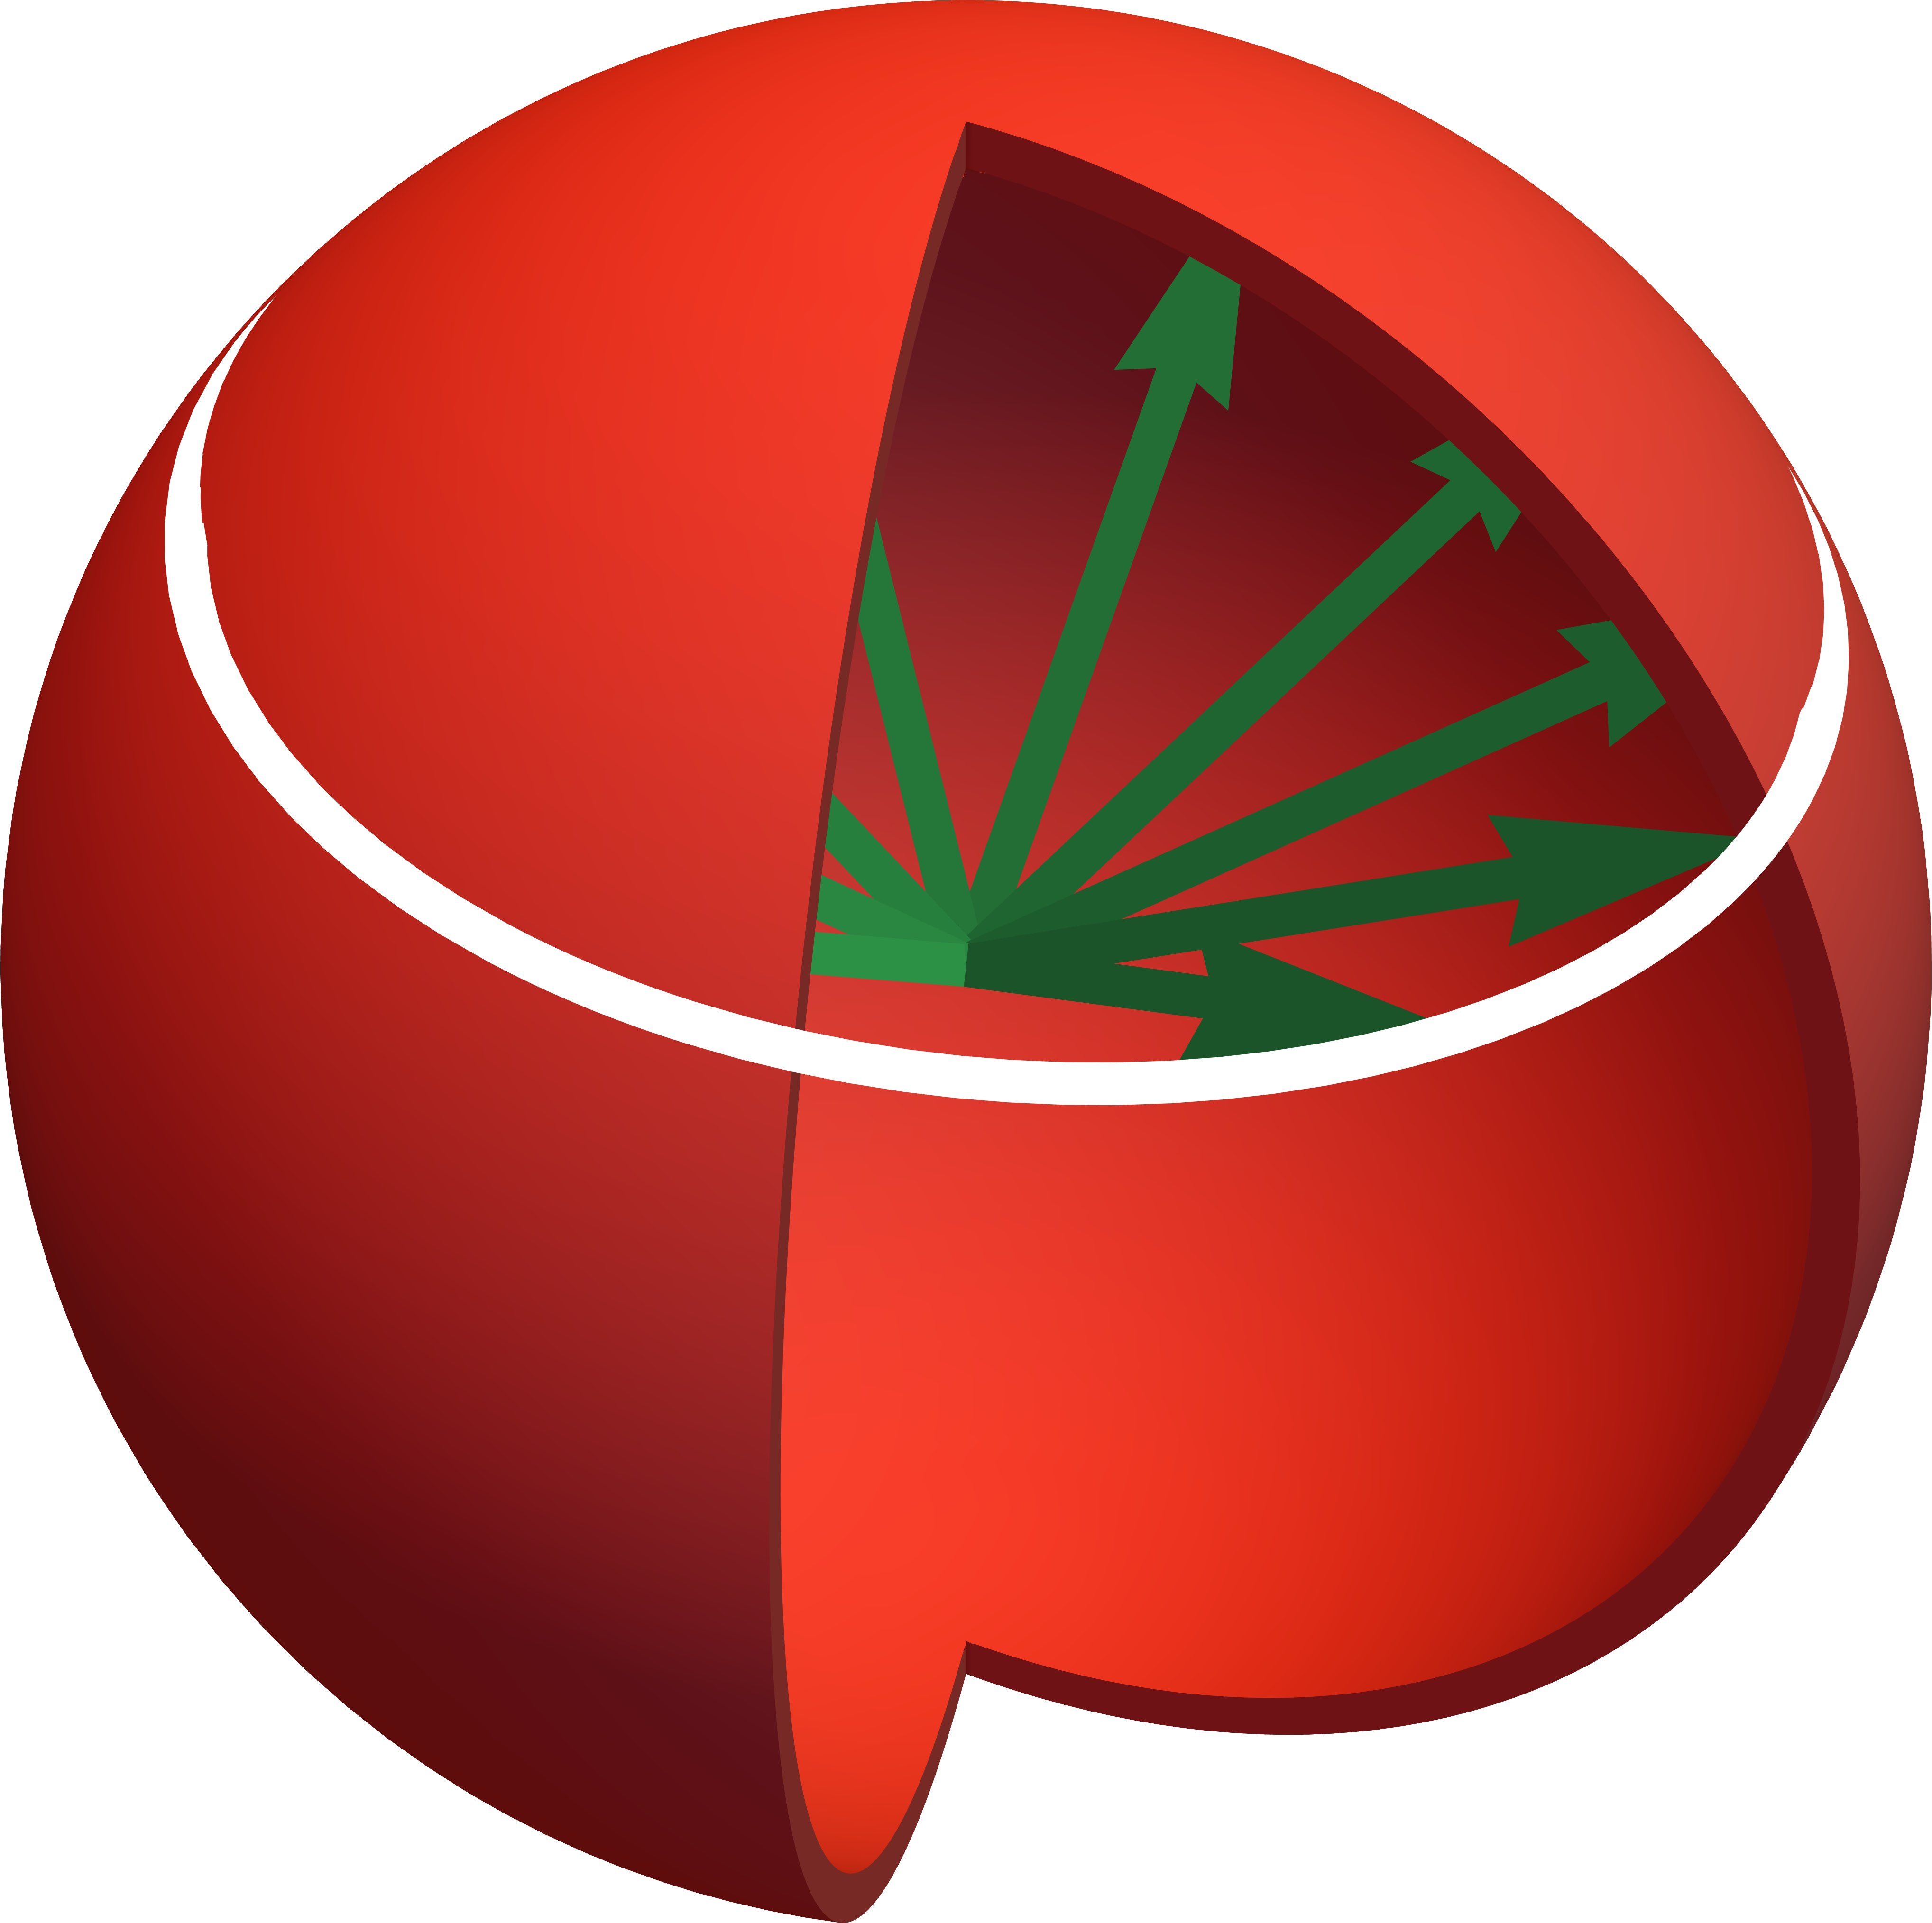
\includegraphics[width=0.13\textwidth]{figures/ssh_deformed_normalized_bloch_vector_t0_825.jpg}
    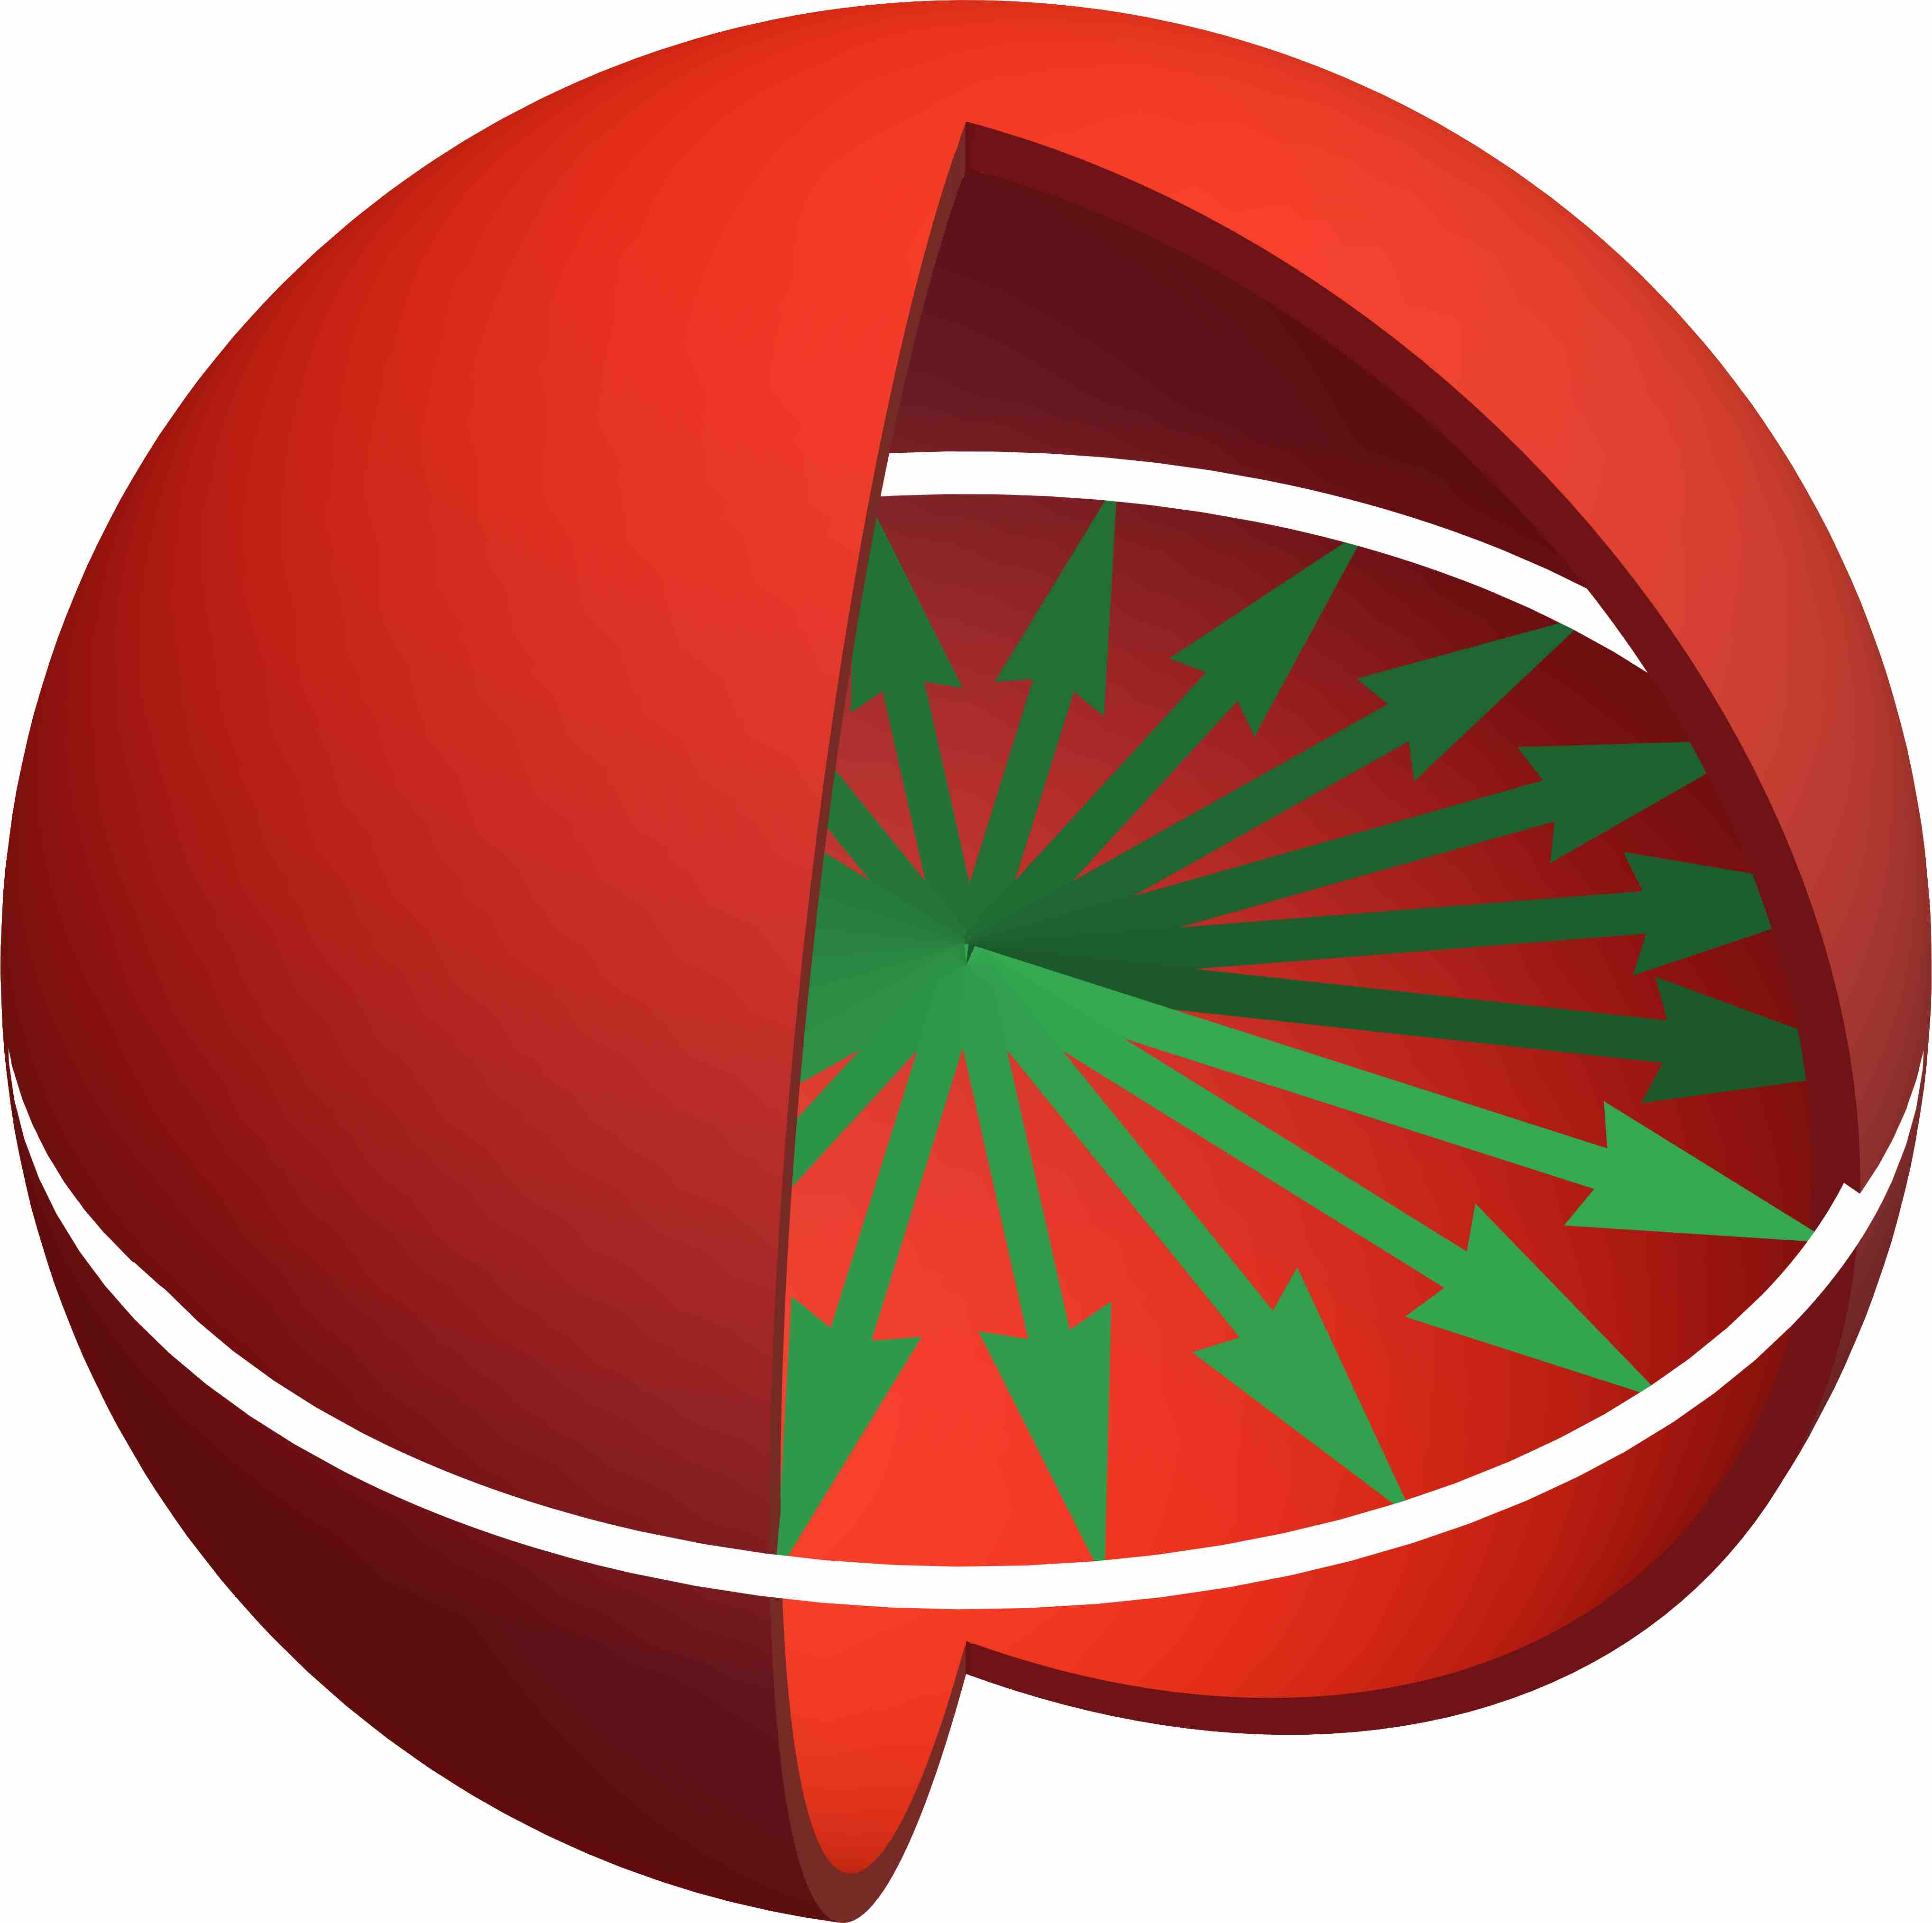
\includegraphics[width=0.13\textwidth]{figures/ssh_deformed_normalized_bloch_vector_t1_000.jpg}
    \caption{Depicted paths of $\hat{\bm B}(t,k)={\bm B}/|{\bm B}|$ (see text) as it wraps around the Brillouin zone $k\in(0,2\pi]$ for different $t\in\{0,1/8,1/4,1/2,3/4,7/8,1\}$ (from left to right). The solid angle of $2\pi$ spanned in the TOI phase (i.e. $t=1$) can be smoothly deformed to the trivial case in the TRI phase (i.e. $t=0$).}
    \label{fig:ssh_deformed}
\end{figure}

In the equations above, $H(0,k)$ describes a TRI and $H(1,k)$ a TOI phase.
The spectrum of $H(t,k)$ is readily solved, and it is easy to verify that $\Delta({t})>0$ for $0\leq t\leq1$.
The path of the normalized Bloch vector $\hat{\bm B}(t,k)$ for different values of the parametrization $t$ is depicted in \cref{fig:ssh_deformed}:
If a deformation along the $z$-axis is allowed, the nontrivial circular path is smoothly connected to a trivial point without closing the bulk gap, demonstrating the adiabatic connection between TOI and TRI phases.

This statement can be geometrically understood by the fact that the single-valued parametrization $\bm B(k)$ generates an arc of a circle or a full circle on the Bloch sphere.
In other words, the surface $S$ spanned by $C$ (the white path in \cref{fig:ssh_deformed}) never fully encapsulates the degeneracy, which is the source of ${\bm F}_n$.
As a consequence, $\gamma_n(C)$ is not quantized and adiabatic deformations like \cref{eq:hamiltonian_path} are possible to effectively remove the degeneracy from the surface integral, smoothly connecting all nonzero geometric phases to the trivial one.
\begin{figure}[ht]
    \centering
    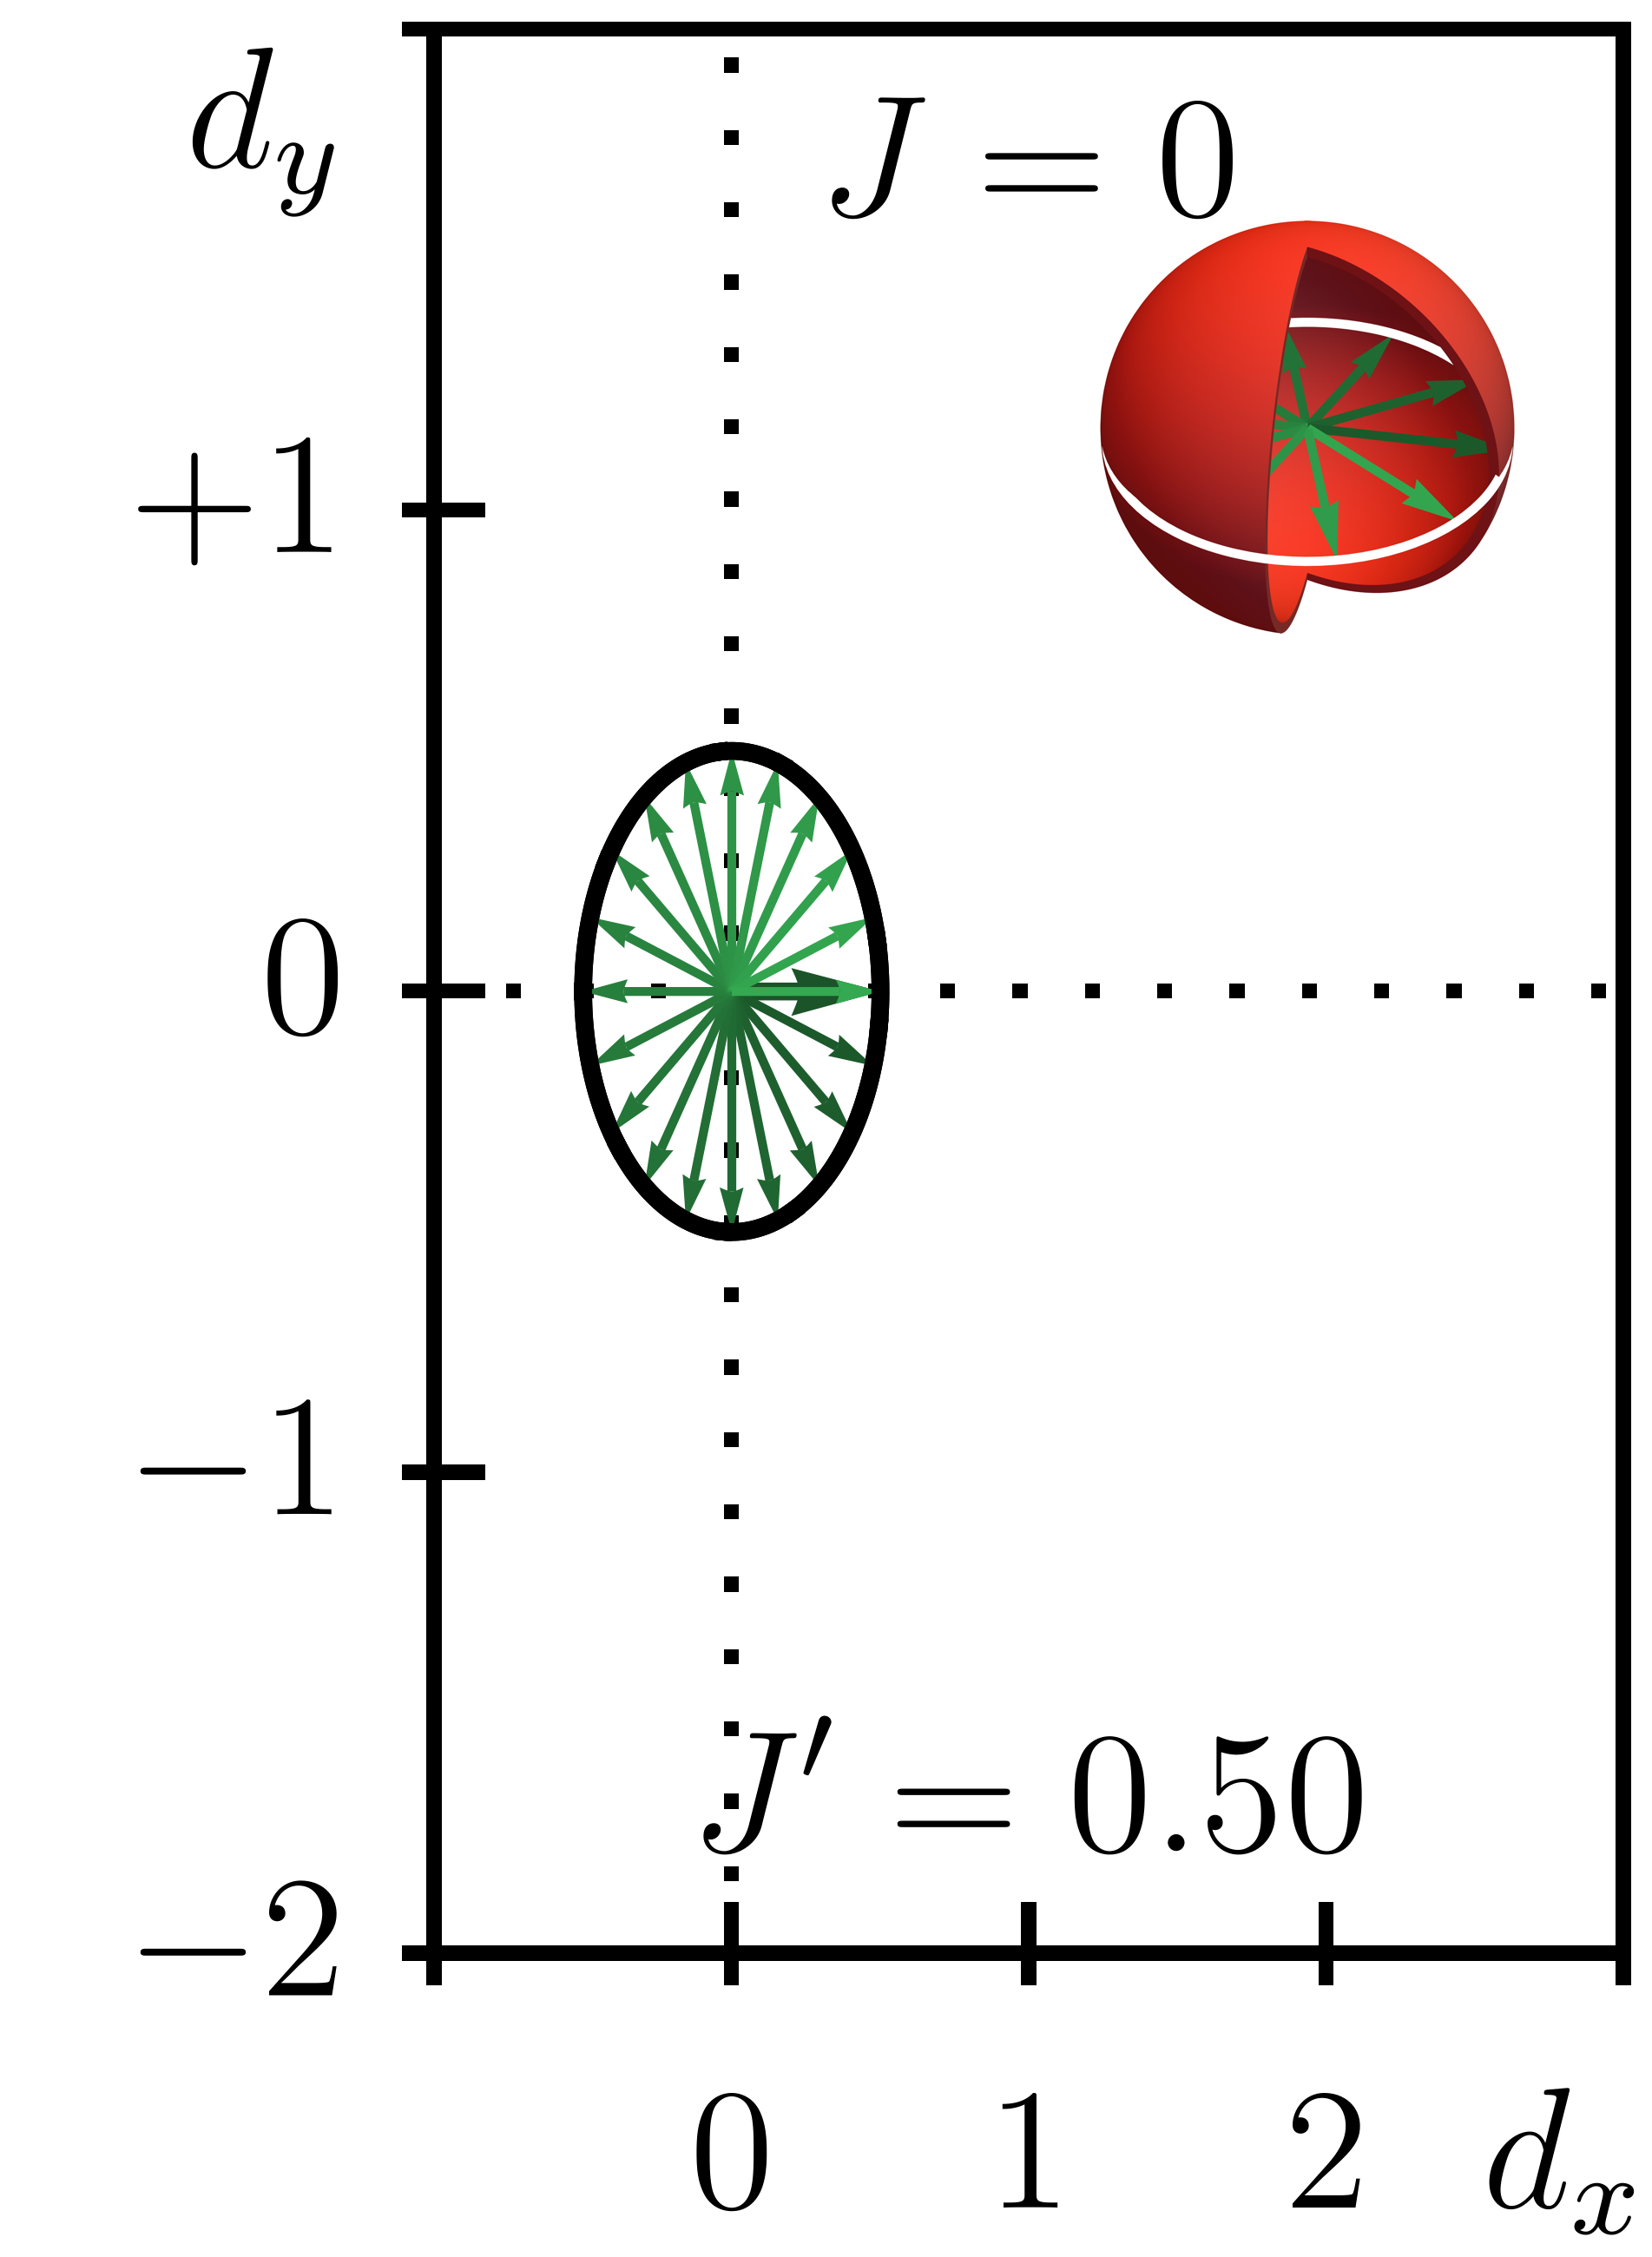
\includegraphics{figures/ssh_unnormalized_winding_2.png}
    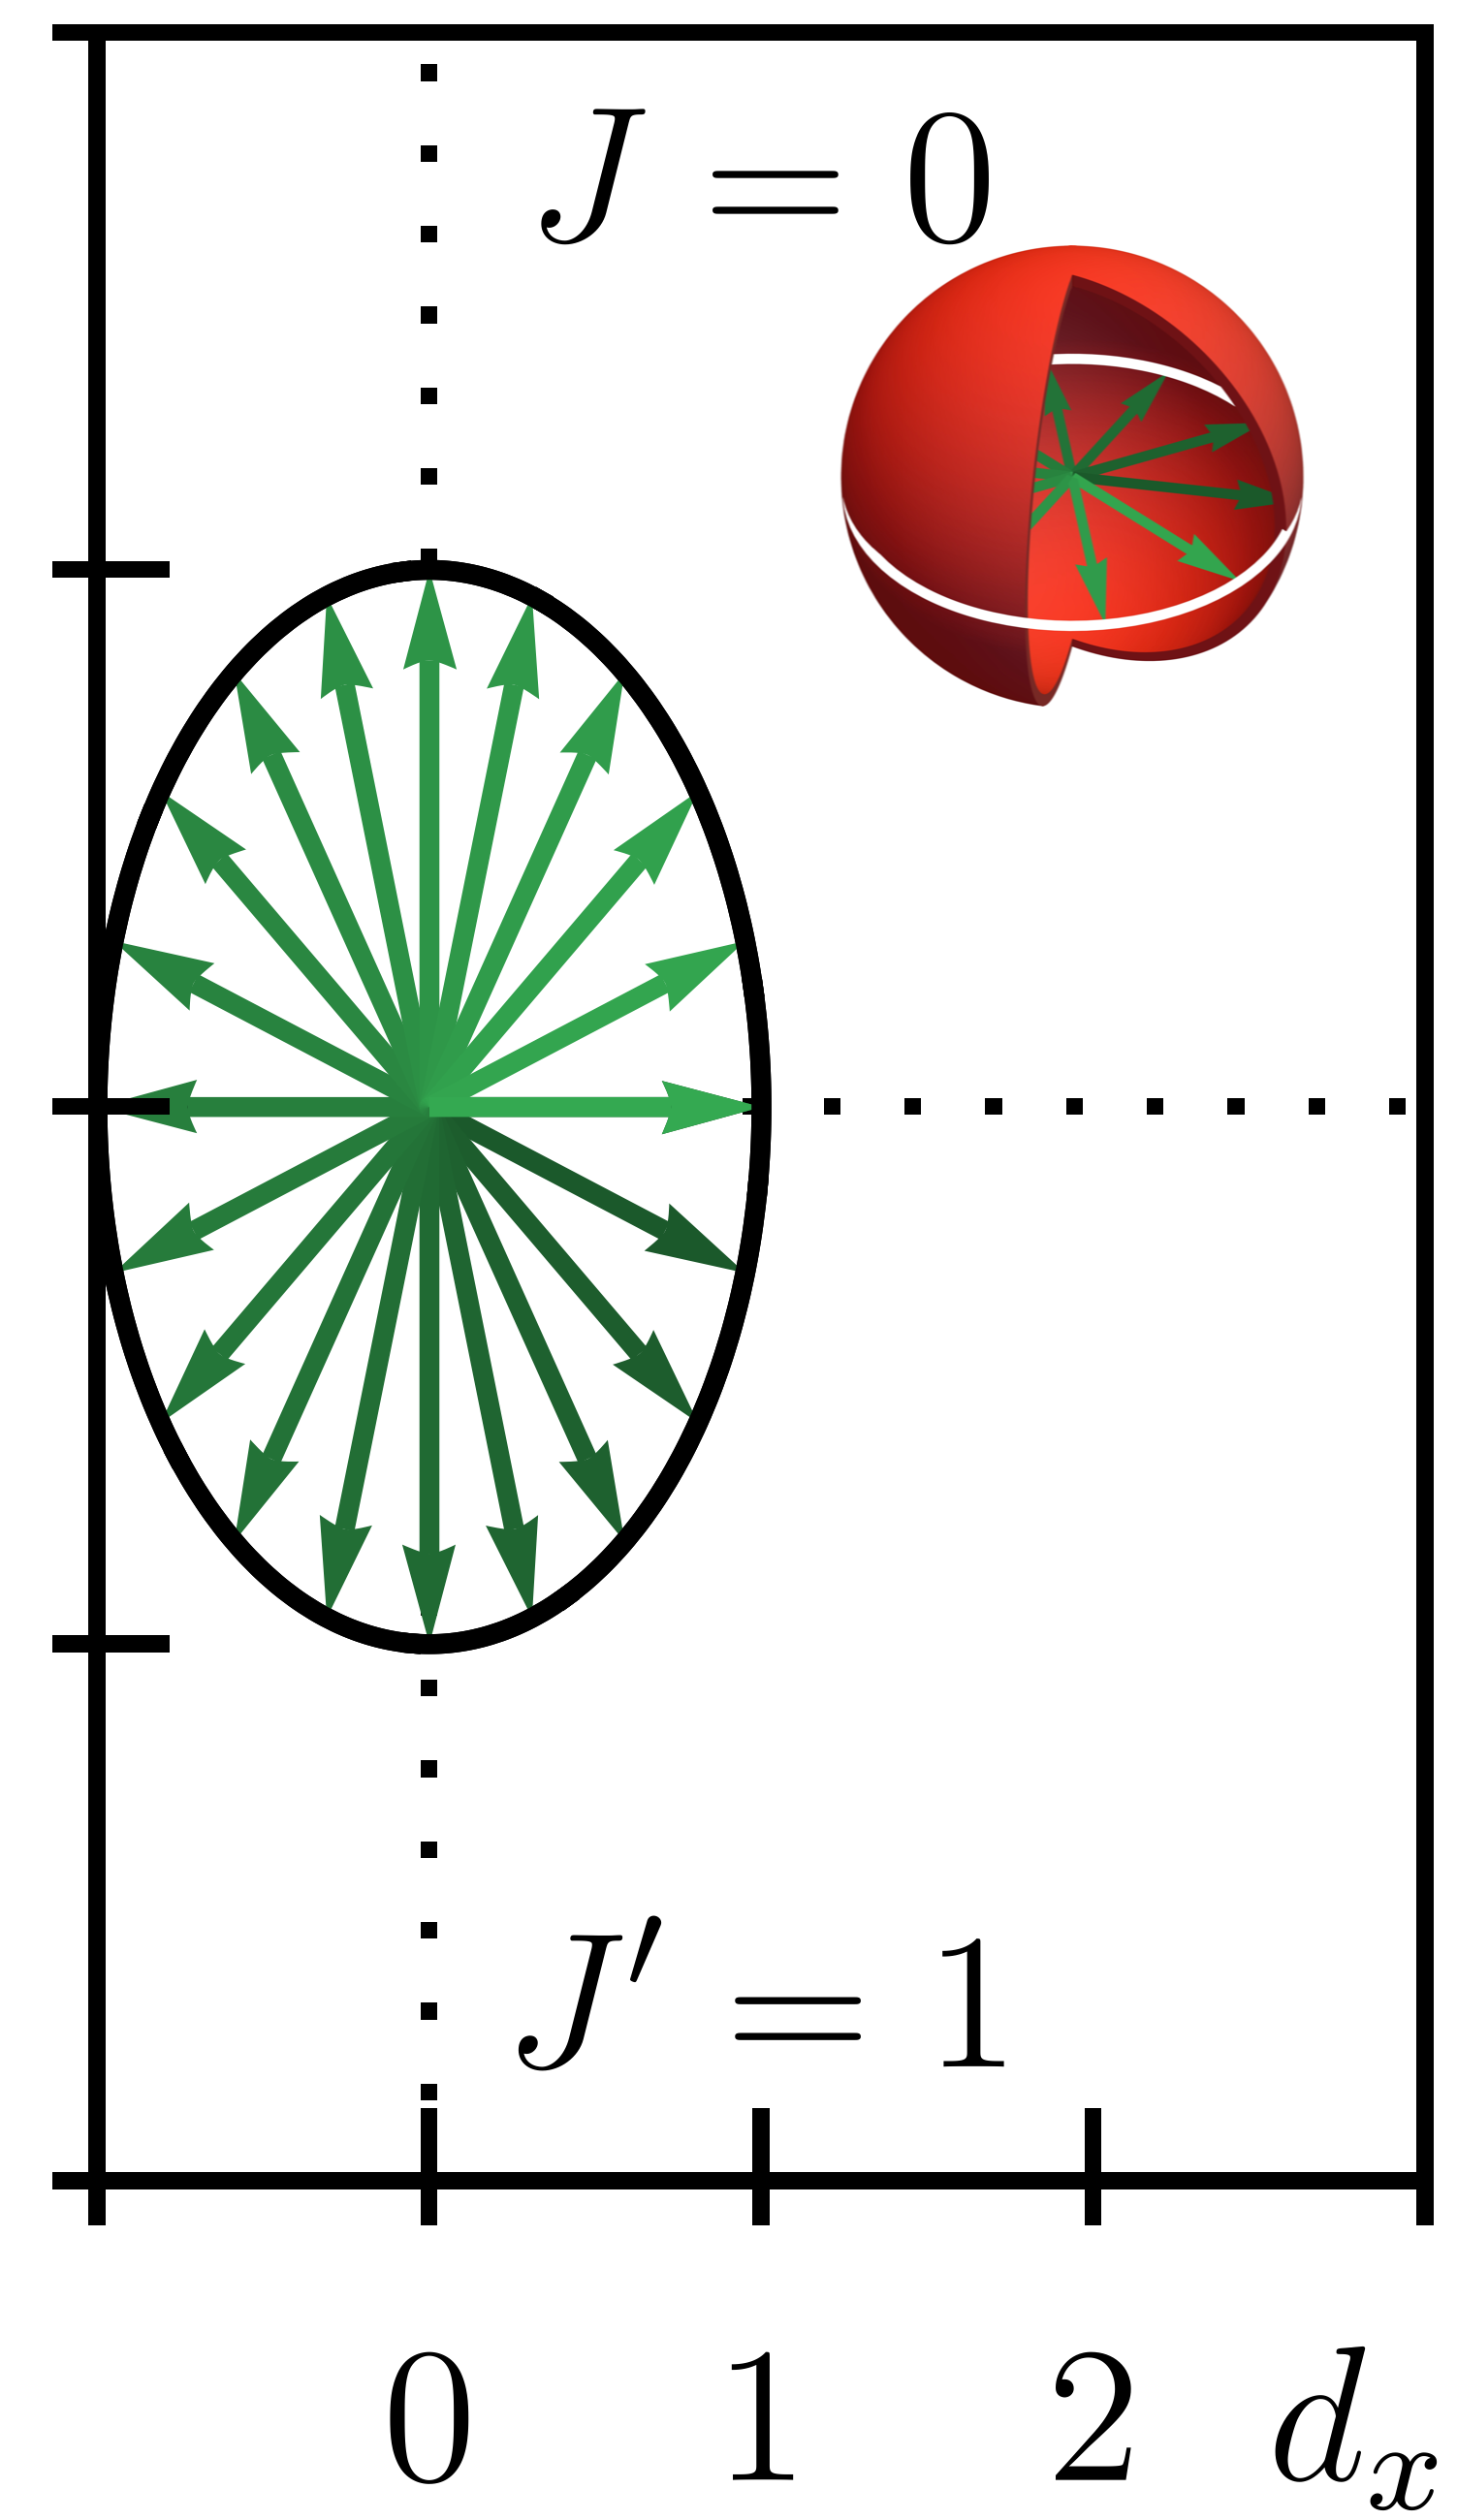
\includegraphics{figures/ssh_unnormalized_winding_3.png}
    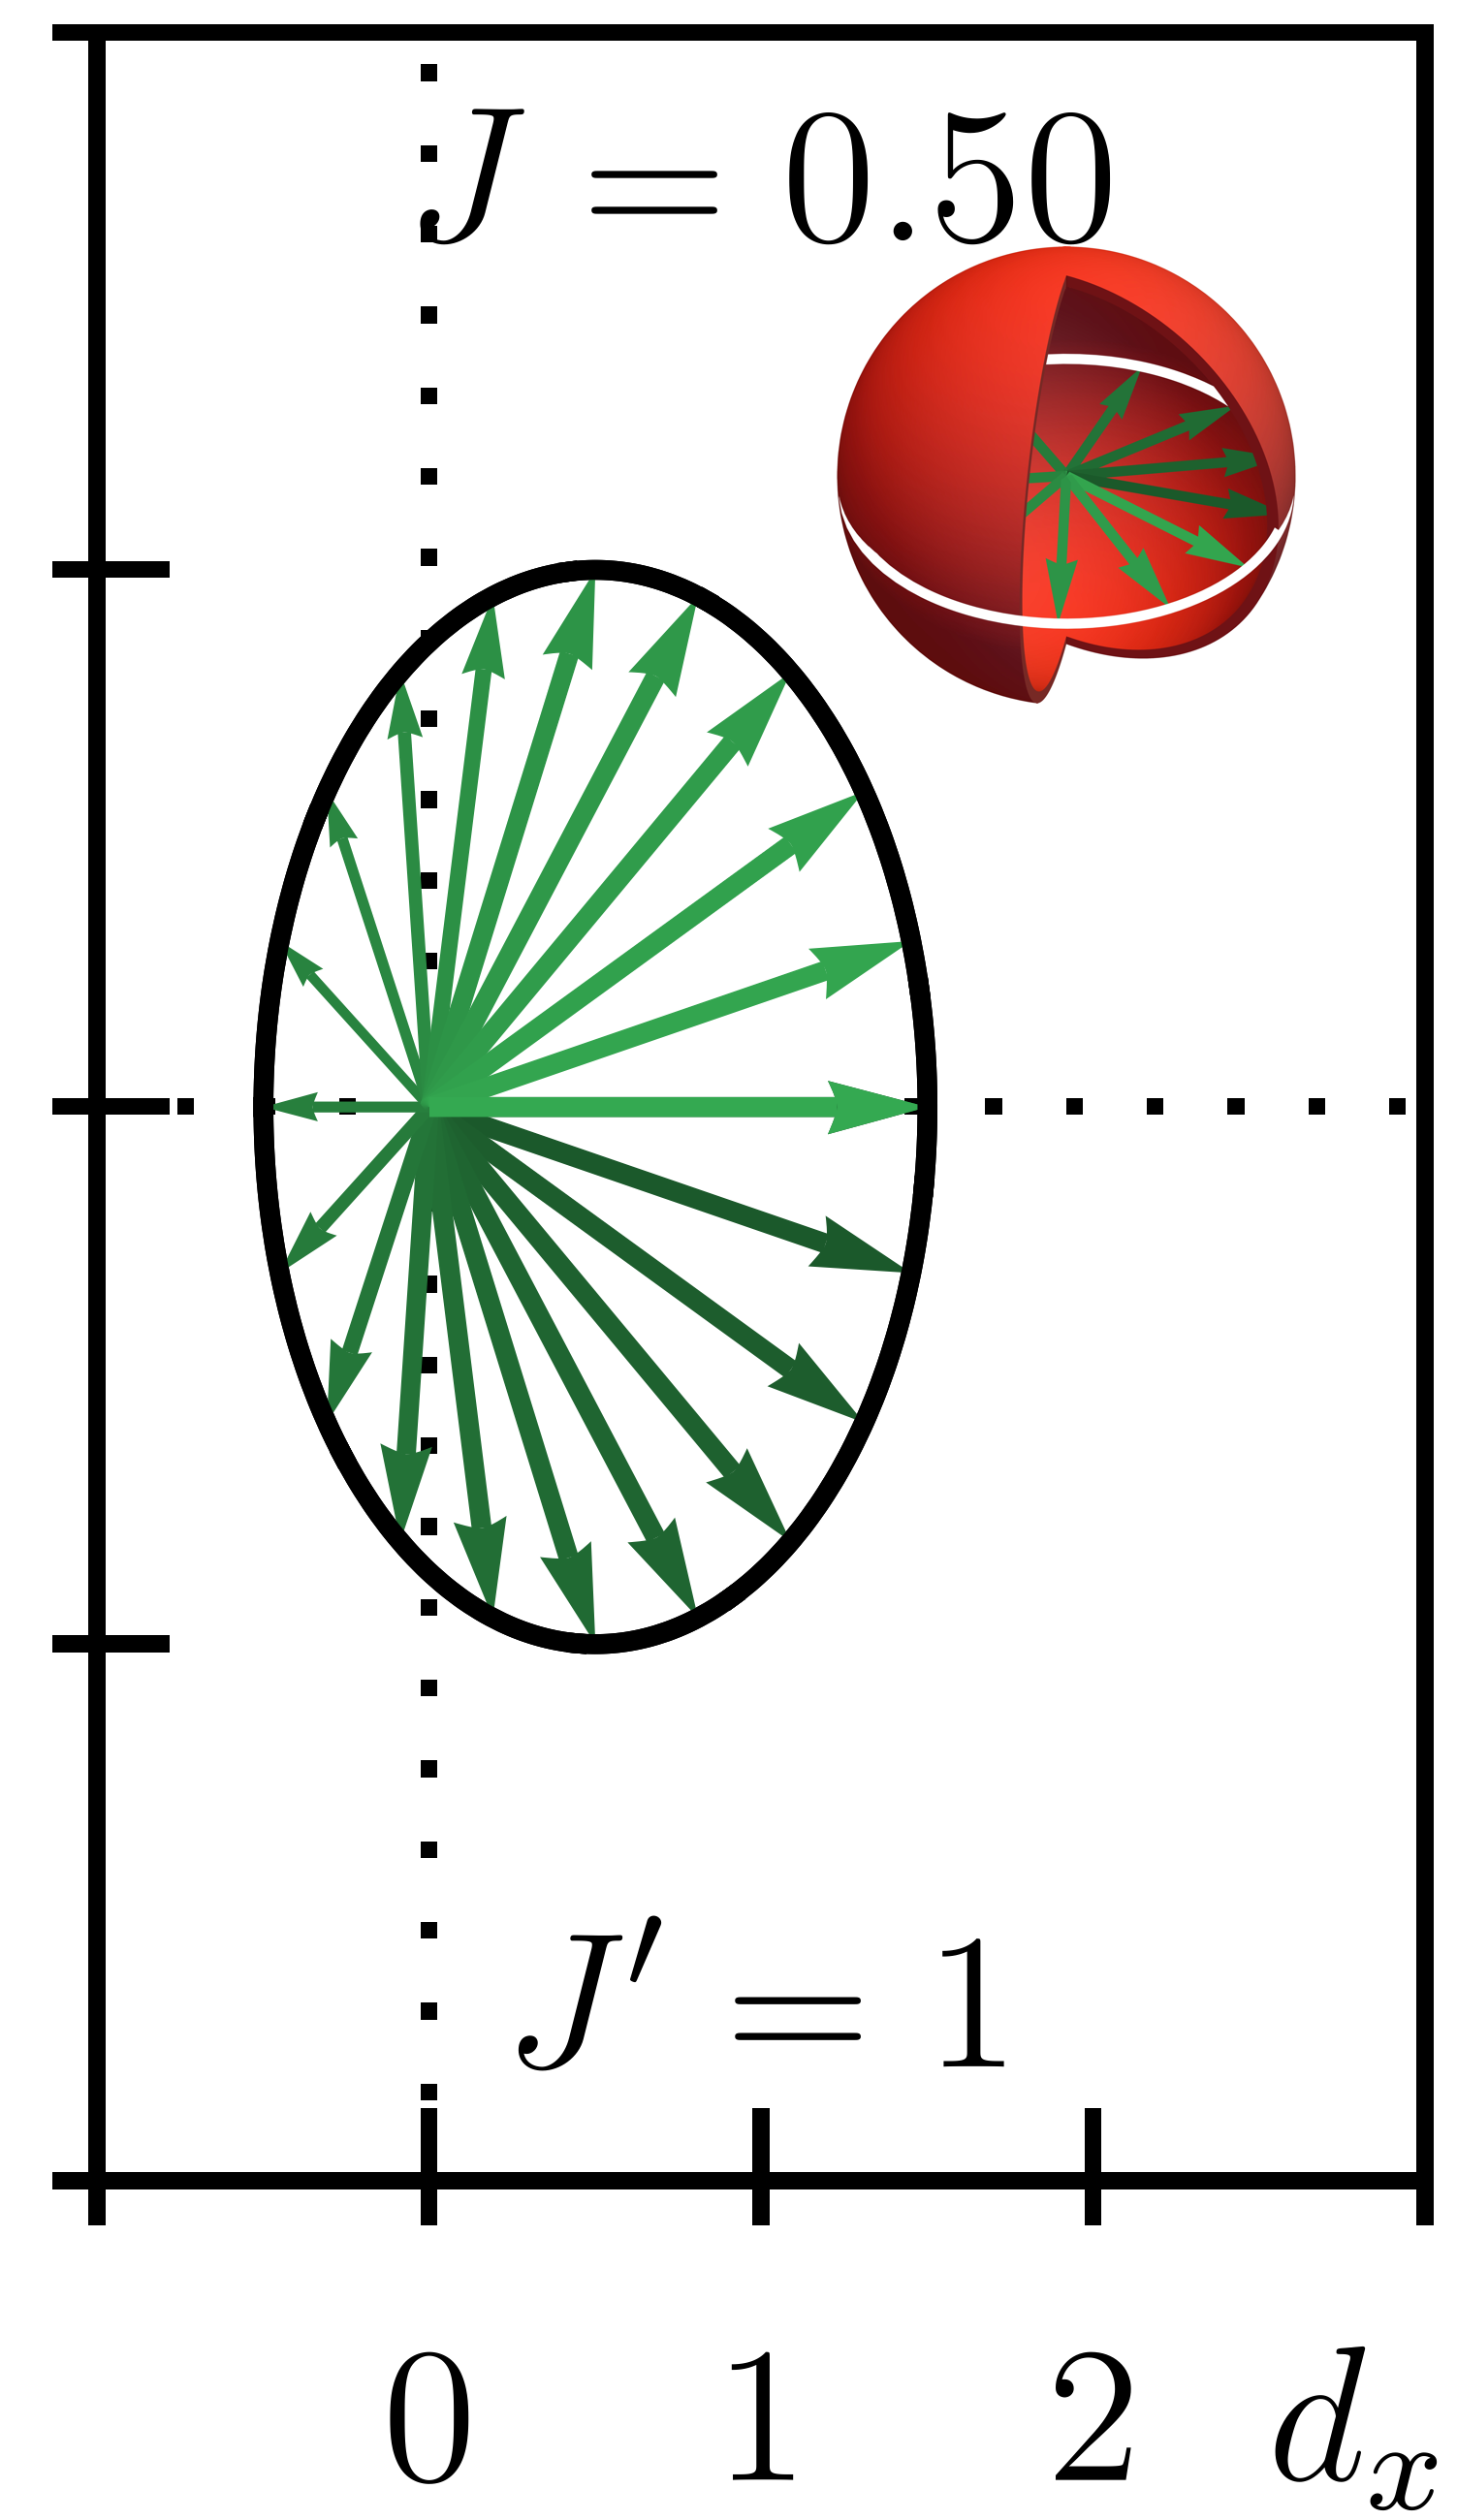
\includegraphics{figures/ssh_unnormalized_winding_4.png}
    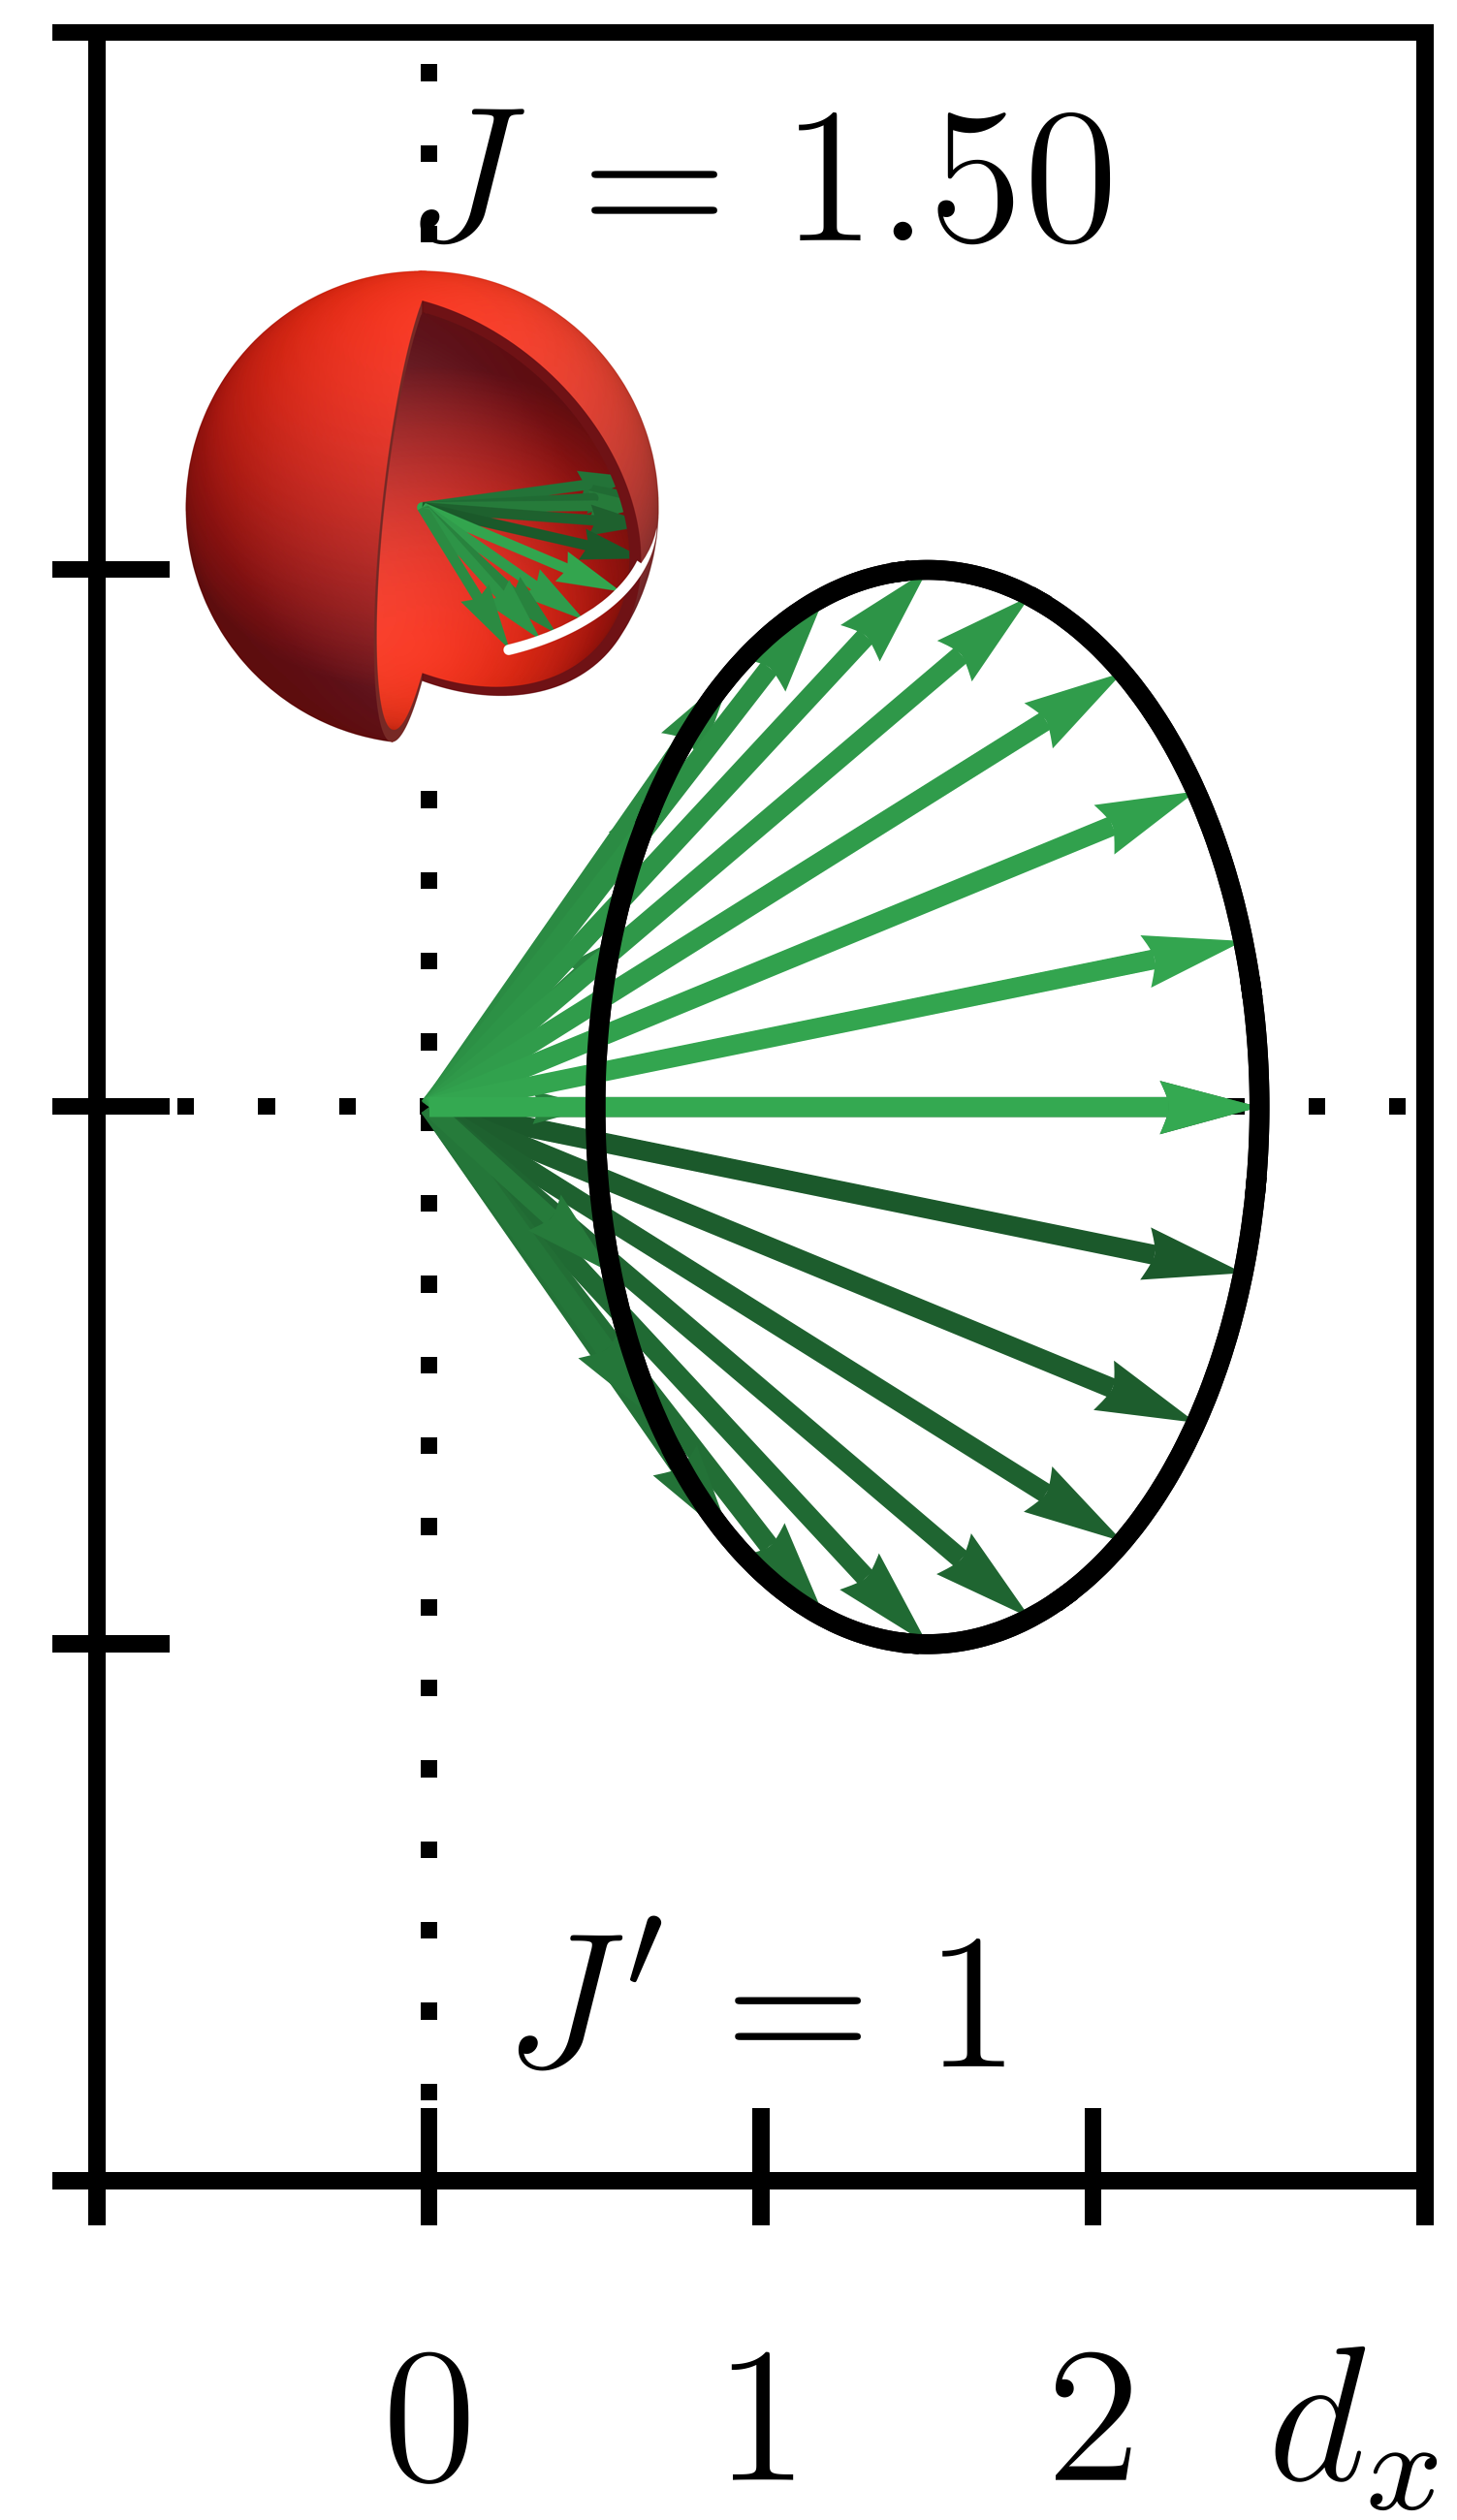
\includegraphics{figures/ssh_unnormalized_winding_6.png}
    \caption{The path in $x,y$ plane spanned by the unnormalized Bloch vector $\bm B$, compared with the path of $\hat{\bm B}$ drawn on the Bloch sphere for different values of $J'/J$. The path drawn by $\bm B$ either traverses around the origin or not, resulting in a path spanning a nonzero surface area or a path which retraces itself thus spanning no surface.}
    \label{fig:ssh_winding_easy}
\end{figure}

If, however, we require to keep $H(t,k)$ entirely off-diagonal, deformations like \cref{eq:hamiltonian_path} with terms $B_z\neq0$ do not exist.
As a consequence, any interpolation from a TOI to a TRI Hamiltonian necessarily crosses the critical point $J=J'$ where the bulk gap vanishes.
The Berry phase of such a system is an element of $\pi\mathds Z$, being non-zero if and only if the path $C$ spanned by $\hat{\bm B}$ defines the boundary of a nontrivial surface.
% This can be understood intuitively:
% By imposing the off-diagonal structure of the family of Hamiltonians, the degeneracy cannot be removed from a nonzero surface integral, and as a consequence the Berry phase is quantized.
In analogy to the Chern number, this defines a topological index called the winding number, which corresponds to quantized values only in the equivalence classes of Hamiltonians respecting the imposed ``symmetry'' of being off-diagonal (this is defined more properly in \cref{sec:Periodic_table_of_topological_insulators_and_superconductors}).
It equals to the Berry phase divided $\pi$, i.e.
\begin{align}
    \mathcal W = |\gamma_n(C)/\pi|,
\end{align}
or, equivalently, to the solid angle spanned by $\hat{\bm B}$ divided $2\pi$, i.e.
\begin{align}
    \mathcal W = \frac1{2\pi}\int\rd k\brlr{\hat{\bm B}\times\partial_k\hat{\bm B}}_z.
\end{align}
Since the winding number counts the amount of full circles $\hat{\bm B}$ performs around the origin while passing through the Brillouin zone, it is equal to
\begin{align}
    \mathcal W = \frac{1}{2\pi}\int\rd k \arg(\hat{\bm B}_x - \ri \hat{\bm B}_y)
    =
    \frac{1}{4\pi\ri} \tr\int\rd k \sigma_z H^{-1}\partial_k H
    =
    \frac{1}{4\pi\ri} \tr\int\rd k \sigma_z g^{-1}\partial_k g,
    \label{eq:winding_number}
\end{align}
in which $g(k)=G(k,\omega=0)$ is the Green's function at zero frequency.

The winding number can most easily be identified by close inspection of the unnormalized Bloch vector ${\bm B}$, traversing (or not) around the degeneracy.
This will then translate to $\hat{\bm B}$ drawing circles around the Bloch sphere, or retracing itself, thus spanning no surface (see \cref{fig:ssh_winding_easy} and compare plots with the insets).
In particular, the former will be achieved if $J<J'$ ($\mathcal W=1$), while the latter occurs for $J>J'$ ($\mathcal W=0$).
From now on, we call a phase with nonzero winding number topological insulator (TOI) and the other trivial insulator (TRI).

To understand the emergence of edge modes, we must obviously introduce an interface of some sort.
First of all, let us Fourier-transform the Bloch Hamiltonian to find the representation in real space, i.e.
\begin{align}
    \hat H = \sum_x \brlr{J\hat c^\dag_{x,A}\hat c^\pdag_{x,B} + J' \hat c^\dag_{x,B}\hat c^\pdag_{x+1,A}} + \hc,
\end{align}
in which $\hat c_{x,A/B}$ are the annihilators of a spinless fermionic particle at site $x$ and sublattice $A/B$.
An interface hosting edge states with energy zero, following the logic of the previous section, is readily implemented by two semi-infinite crystals, one with bulk invariant $0$ (e.g. for all negative lattice positions $x<0$), the other with bulk invariant $1$ (for all lattice positions $x\geq0$).
For convenience, let us construct this crystal from the two limiting cases (i) $J'=0$ and (ii) $J=0$.
Note that for such a system, the central $A$ site at position $x=0$ does not contribute to the Hamiltonian and hosts a perfectly localized mode of zero energy.
Obviously, this edge mode is preserved if we consider the vacuum in region (i).
Let us simplify the hypothetical crystal by replacing the trivial insulator with the vacuum, and proceed by relaxing the constraint $J=0$ to $J'>J$ on the semi-infinite crystal:
\begin{align}
    \hat H = \sum_{x\geq0} J \hat c^\dag_{x,A}\hat c^\pdag_{x,B} + J' \hat c^\dag_{x,B}\hat c^\pdag_{x+1,A} + \hc
\end{align}
In this case, the presence of an edge zero mode is not particularly obvious and requires further inspection.
One observation is that the fermionic Hamiltonian can be diagonalized by unitary transformations, which requires only a diagonalization of $\hat H = \hat{\bm c}^\dag H \hat{\bm c}$, where $\hat{\bm c}=(\hat c_{0,A},\hat c_{0,B},\hat c_{1,A},\hat c_{1,B},\dots)^T$ is the successive vector of all fermionic annihilation operators.
The matrix $H$ is quite sparse and has only alternating off-diagonal elements
\begin{align}
    H =
    \begin{pmatrix}
        0 & J & 0 & 0 &\dots \\
        J & 0 & J' & 0 & \dots \\
        0 & J' & 0 & J & \dots \\
        0 & 0 & J & 0 & \dots \\
        \vdots & \vdots & \vdots & \vdots & \ddots
    \end{pmatrix},
\end{align}
such that an analytic treatment is not too difficult, even if the entries are spatially dependent~\cite{Asboth2016}.
An exact boundary mode can be found by evaluating $hv_L=0$, with a vector $v_L = (a_0,b_0,a_1,b_1,\dots)^T$, resulting in the set of equations
\begin{align}
    J b_0 = 0,
    \quad
    Ja_m + J' a_{m+1} = 0,
    \quad
    J' b_m + J b_{m+1} = 0.
\end{align}
Defining $w=J'/J$, the solution reveals an exponentially localized zero energy mode with no support on sublattice $B$, i.e.
\begin{align}
    a_k=(-w)^{-k} a_0 \rightarrow |a_k| = \re^{-k/\ln w}|a_0|,
    \quad
    b_k = 0.
    \label{eq:boundary_mode}
\end{align}
It is also transparent that the state generated by the vector $v_L$ would violate normalization in the TRI phase ($w<1$) and is thus allowed to exist only if the geometric series is convergent.

In case of a finite crystal with $N$ sites, a similar reasoning reveals the existence of two such boundary modes, generated by the vectors $v_L$ and $v_R$.
Similarly to $v_L$, $v_R$ is exponentially localized at the right interface, has no support on sublattice $A$ and decays exponentially into the bulk.
Thus, the two modes share exactly no overlap $v_L^T v_R = 0$.
However, the two modes are not exact eigenstates of the Hamiltonian since each one slightly violates the boundary conditions.
Note that $v_{L/R}^T h v_{L/R} = 0$ and $v_{L/R}^T h v_{R/L} = (1-w^{-1})^{-1}\re^{-(N-1)/\ln w}\re^{\pm\ri\varphi}$ with some phase $\varphi$.
This then yields ``state hybridization'': a pair of orthogonal eigenstates $v_\pm = 1/\sqrt2(v_L \pm v_R\re^{\pm\ri\varphi})$ with energy $\pm(1-w^{-1})^{-1}\re^{-(N-1)/\ln w}$.
Therefore, the hybridized states are exponentially localized boundary modes and of ``almost'' zero energy with an exponentially small splitting in the system size.
%
%
%%%%%%%%%%%%%%%%%%%%%%%%%%%%%%%%%%%%%%%%%%%%%%%%%%%%%%%%%%%%%%%%%%%%%%%%
\section{Periodic table of topological insulators and superconductors}
\label{sec:Periodic_table_of_topological_insulators_and_superconductors}
%%%%%%%%%%%%%%%%%%%%%%%%%%%%%%%%%%%%%%%%%%%%%%%%%%%%%%%%%%%%%%%%%%%%%%%%
%
%
Let us consider an arbitrary non-interacting system of fermions, described by the particle-number conserving Hamiltonian
\begin{align}
    \hat H = \sum_{i,j}\hat c^\dag_{i}H_{ij}\hat c^\pdag_j = \hat{\bm c}^\dag H \hat{\bm c}^\pdag
\end{align}
with a matrix $H$ dictating possible transition events.
As before, we denote the collection of the fermionic operators as $\hat{\bm c}$.
Note that $i,j$ are generic index labels -- they may represent a combination of the position $\bm x_i$ and additional ``internal quantum numbers'' $i\coloneqq(\bm x_i,q_i)$, e.g. the sublattice index $q_i\in \{A,B\}$ of the SSH model.
The system is invariant under a (unitary) symmetry transformation $\hat U$, if it acts on the fermionic annihilation operators as a linear map
\begin{align}
    \hat{\bm c}\rightarrow \hat{\bm c}' = \hat U \hat{\bm c} \hat U^{-1} = U \hat{\bm c},
\end{align}
such that the canonical anticommutation relations and $\hat H$ are preserved, i.e.
\begin{align}
    \hat U\anticommutator{\hat c_i^\pdag,\hat c_j^\dag}\hat U^{-1}
    =
    \anticommutator{\hat c_i^\pdag,\hat c_j^\dag}
    \rightarrow
    U^\dag U = \mathbb1
    ,\quad
    \hat U \hat H \hat U^{-1} = \hat H
    \rightarrow
    U^\dag H U = H
    .
\end{align}
Focussing on the so-called ``Altland-Zirnbauer'' classification scheme, we consider here on-site symmetries only~\cite{Altland1997}.
On-site symmetries, as the name suggests, only act on the ``internal'' degrees of freedom, such that they can be factorized $\hat U=\prod_{\bm x}\hat V_{\bm x}$ with the same $\hat V_{\bm x}$ on all lattice positions.
Please note that $\hat V_{\bm x}$ acts nontrivially only on the ``internal dimension''.

{\it 1. Time reversal symmetry} Recall that anti-unitary transformations can be written as a composition of complex conjugation with unitary transformations\footnote{Note that $\hat c\rightarrow \hat c^\dag$ in \cref{eq:time_reversal_symmetry} would be an equally valid choice, but this is treated by convention as a combination of time reversal and particle hole symmetry.}, i.e.
\begin{align}
    \hat T \hat c_i \hat T^{-1} = {U_T}_{ij} \hat c_j
    ,\quad
    \hat T\ri\hat T^{-1}=-\ri
    ,\quad
    {U_T}^\dag H^* U_T = H.
    \label{eq:time_reversal_symmetry}
\end{align}
Applying the transformation twice results in the condition
\begin{align}
    H = {U_T}^\dag ({U_T}^\dag H^* U_T)^* U_T = ({U_T}^*U_T)^\dag H ({U_T}^* U_T).
\end{align}
Since the first quantized Hamiltonian runs over an irreducible representation space, ${U_T}^* U_T = \re^{\ri\alpha}\mathbb1$ due to Schur's lemma~\cite{Chiu2016}.
Moreover, $U_T$ is a unitary matrix, satisfies ${U_T}^*={U_T}^\dag\re^{\ri\alpha}$ (and equally ${{U_T}^\dag}^* = U_T\re^{\ri\alpha}$), and $({U_T}^\dag U_T)^* = \re^{-\ri2\alpha}\mathbb1$, for which $\alpha\in\pi\mathds Z$.
This implies that
\begin{align}
    \hat T^2 \hat c_i \hat T^{-2} = {U_T}_{ij}^*{U_T}_{jk} \hat c_k = \re^{\ri\alpha}\hat c_i
\end{align}
maps to itself up to a possible sign.
$\hat T$ acts on-site only and therefore a generic $n$-body operator $\hat O$ transforms to $\hat T^2\hat O \hat T^{-2} = \re^{\ri\alpha n}\hat O$, which leads to
\begin{align}
    \hat T^2 = (\pm 1)^{\hat N}\Leftrightarrow {U_T}^* {U_T} = \pm\mathbb1,
\end{align}
with $\hat N = \sum_i \hat c^\dag_i \hat c^\pdag_i$.
In case of $\hat T^2=-1$ (e.g. for systems with an odd number of electrons), this then yields the famous Kramers degeneracy of the eigenvalues~\cite{Schwabl2007}.

{\it 2. Particle-hole symmetry} is unitary and relates creation to annihilation operators, i.e.
\begin{align}
    \hat C \hat c_i \hat C^{-1} = {U_C}^*_{ij} \hat c^\dag_j
    ,\quad
    {U_C}^\dag H^* {U_C} = -H
    .
\end{align}
Such systems are characterized by off-diagonal quadratic Hamiltonians $\tr H=0$.
Repetition of the previous computation yields
\begin{align}
    \hat C^2 = (\pm1)^{\hat N}
    \Leftrightarrow
    {U_C}^* {U_C} = \pm 1.
\end{align}

{\it 3. Chiral symmetry} is the combination of $\hat T$ with $\hat C$ to a so-called chiral symmetry
\begin{align}
    \hat S = \hat T \hat C.
\end{align}
This may lead to a situation where both time reversal and particle-hole symmetry do not hold, but chiral symmetry is satisfied.
One finds
\begin{align}
    \hat S \hat c_i \hat S^{-1} = (U_CU_T)_{ij}\hat c^\dag_j
    ,\quad
    {U_S}^\dag H {U_S} = -H
    ,\quad
    {U_S} = {U_C}^* {U_T}^*
    ,
\end{align}
in which, contrary to the other two symmetries, $U_S^2=\re^{\ri\alpha}\mathbb1$.
This leaves a phase ambiguity that is fixed by $U_S\rightarrow U_S\re^{\ri\alpha/2}$ such that the eigenvalues of the chiral operator are gauged to $\pm1$.

The established terminology allows to discuss the general symmetry classification of non-interacting systems.
We obtained so far
\begin{align}
    \begin{array}{l l l l }
        & T^{-1}HT = +H
        ,\quad
        & T = U_T\mathcal K
        ,\quad
        & U_T^*U_T = \pm\mathbb1,\\
        %
        & C^{-1}HC = -H
        ,\quad
        & C = U_C\mathcal K
        ,\quad
        & U_C^*U_C = \pm\mathbb1,\\
        %
        & S^{-1}HS = -H
        ,\quad
        & S = U_S = U_C^* U^*_T
        ,\qquad
        & U_S^2 = \mathbb1.
    \end{array}
    \label{eq:symmetry_real_space}
\end{align}
The set of symmetries $\hat T$, $\hat C$ and $\hat S$ is exhaustive and spans the ten possible families of Hamiltonians as presented in \cref{tab:symmetry_classes}~\cite{Chiu2016}.
Consider the case of time reversal invariance, there are three distinct classes:
(i) $H$ is not time reversal invariant, denoted by $T=0$, (ii) $H$ is time reversal invariant and $T$ squares to $+\mathbb1$ in which case we write $T=+$ and (iii) $H$ is time reversal invariant and $T$ squares to $-\mathbb1$, denoted by $T=-$.
There are three equivalent ways to characterize the behavior of $H$ under the particle hole symmetry.
Since $\hat S = \hat C\hat T$ in eight of the nine previous possibilities the outcome of chiral symmetry is implied.
However, the Hamiltonian can (or cannot) be chiral invariant in the absence of $C$ and $T$ symmetry, such that there are ten distinct symmetry classes.

\begin{table}
    \centering
    \addtolength{\tabcolsep}{0.25cm}
    \renewcommand{\arraystretch}{1.25} % 1 standard
    \begin{tabular}{l | c c c | l l l l l l l l l}
        \hline\hline
        Class   & $T$ & $C$ & $S$ & $0$ & $1$ & $2$ & $3$ & $4$ & $5$ & $6$ & $7$ & $8$\\
        \hline
        A       & $0$ & $0$ & $0$ & $\mathds Z$   &               & $\mathds Z$   &               & $\mathds Z$   &               & $\mathds Z$   &               & $\mathds Z$   \\
        AIII    & $0$ & $0$ & $+$ &               & $\mathds Z$   &               & $\mathds Z$   &               & $\mathds Z$   &               & $\mathds Z$   &               \\
        \hline
        AI      & $+$ & $0$ & $0$ & $\mathds Z$   &               &               &               & $2\mathds Z$  &               & $\mathds Z_2$ & $\mathds Z_2$ & $\mathds Z$   \\
        BDI     & $+$ & $+$ & $+$ & $\mathds Z_2$ & $\mathds Z$   &               &               &               & $2\mathds Z$  &               & $\mathds Z_2$ & $\mathds Z_2$ \\
        D       & $0$ & $+$ & $0$ & $\mathds Z_2$ & $\mathds Z_2$ & $\mathds Z$   &               &               &               & $2\mathds Z$  &               & $\mathds Z_2$ \\
        DIII    & $-$ & $+$ & $+$ &               & $\mathds Z_2$ & $\mathds Z_2$ & $\mathds Z$   &               &               &               & $2\mathds Z$  &               \\
        AII     & $-$ & $0$ & $0$ & $2\mathds Z$  &               & $\mathds Z_2$ & $\mathds Z_2$ & $\mathds Z$   &               &               &               & $2\mathds Z$  \\
        CII     & $-$ & $-$ & $+$ &               & $2\mathds Z$  &               & $\mathds Z_2$ & $\mathds Z_2$ & $\mathds Z$   &               &               &               \\
        C       & $0$ & $-$ & $0$ &               &               & $2\mathds Z$  &               & $\mathds Z_2$ & $\mathds Z_2$ & $\mathds Z$   &               &               \\
        CI      & $+$ & $-$ & $+$ &               &               &               & $2\mathds Z$  &               & $\mathds Z_2$ & $\mathds Z_2$ & $\mathds Z$   &               \\
        \hline\hline
    \end{tabular}
    \addtolength{\tabcolsep}{-0.25cm}
    \caption{The ten symmetry classes of topological insulators and superconductors, sorted by time reversal, particle-hole and chiral symmetry~\cite{Altland1997}, and to which values the unitary transformation of the symmetry squares to. A ``$0$'' indicates absence of the corresponding symmetry while $\pm$ represents the outcome of the squared symmetry transformation (see text). The sets $\mathds Z$, $\mathds Z_2$ and $2\mathds Z$ indicate the existence of topological insulators / superconductors for the corresponding Hamiltonian equivalence class defined in a given space dimension (presented from $0$ to $8$) and which values the topological invariant can assume (integer numbers $\mathds Z$, two distinct numbers $\mathds Z_2$ and even integer numbers $2\mathds Z$).}
    \label{tab:symmetry_classes}
\end{table}

Coming back to the adiabatic principle for gapped Hamiltonians, the topological distinction is defined through smooth deformations of the phase diagram by changing its parameters.
If two quantum systems can be smoothly deformed into each other without closing the gap, they are called topologically equivalent.
Trivial insulators (TRI) are then such phases which are adiabatically connected to an atomic insulator, fully characterized by independent and disconnected unit-cells.
All the other equivalence classes are by definition not adiabatically connected to the atomic insulator and thus called topological insulators (TOI).
To use notation of the previous paragraphs, we decouple the space from the internal dimension, i.e. $H_{ij}=H_{q_1,q_2}(\bm x,\bm x')$ and consider translational invariant systems such that $H_{q_1,q_2}(\bm x,\bm x')=H_{q_1,q_2}(\bm x-\bm x')$.
It is then particularly convenient to use the Bloch Hamiltonian description ($\hat c_{\bm x,q}=\sum_{\bm k}\exp(i\bm k\bm x)\hat c_{{\bm k},q}$), such that the previous Hamiltonian results to
\begin{align}
    \hat H = \sum_{\bm k\in {\rm BZ}} \hat c^\dag_{{\bm k},q} H_{qq'}(\bm k)\hat c^\pdag_{{\bm k},q'},
\end{align}
with the crystal momentum $\bm k$ defined in the first Brillouin zone (BZ).
By close inspection of \cref{eq:symmetry_real_space}, the actions of the symmetries on the Bloch Hamiltonian are given by
\begin{align}
    \begin{array}{l l l l }
        & TH(\bm k)T^{-1} = +H(-\bm k)
        ,\quad
        & T = U_T\mathcal K
        ,\quad
        & U_T^*U_T = \pm\mathbb1,\\
        %
        & CH(\bm k)C^{-1} = -H(-\bm k)
        ,\quad
        & C = U_C\mathcal K
        ,\quad
        & U_C^*U_C = \pm\mathbb1,\\
        %
        & SH(\bm k)S^{-1} = -H(\bm k)
        ,\quad
        & S = U_S = U_C^* U^*_T
        ,\qquad
        & U_S^2 = \mathbb1.
    \end{array}
    \label{eq:symmetry_momentum_space}
\end{align}
The result of the classification is called the periodic table of topological insulators (and superconductors)~\cite{Kitaev2009,Qi2008,Ryu2010,Schnyder2008} and presented in \cref{tab:symmetry_classes}\footnote{The concepts illustrated in this section hold equally for Bogoliubov-de Gennes Hamiltonians, which describe the mean-field theory of a conventional superconductor. Such systems, however, do not make much contact to our published articles, which is why we decided to avoid their notion at this point. Instead, we refer the interested reader to~\cite{Chiu2016,Asboth2016} and the online course \cite{topocondmat}.}.

% \todoil{Unfortunately, this paragraph comes too short and imprecise. Reformulate.}
The table is based on a classification of the vector space of the matrix $\exp(-\ri t H)$, constrained by the presence (or absence) of the symmetries defined by \cref{eq:symmetry_momentum_space}.
For instance, $T=C=S=0$ imposes no additional constraint and the classifying space of the symmetry space $A$ is that of generic unitary matrices of size $N$, i.e. $U(N)$.
This connects to a fundamental work on symmetric space from 1926 by Élie Cartan, and the ten Hamiltonian equivalence classes are in one-to-one correspondence with the ten large families of symmetric spaces~\cite{Heinzner2005}.
Ultimately, it unveils a diagonal structure of the topological index in \cref{tab:symmetry_classes}, in correspondence to the so-called ``Bott clock'', representing a recursive and periodic sequence for the symmetry classes.
In order to see this structure, the table is ordered in a particular manner: the first two rows are spanned by the two classes spanned by complex matrices, whereas the remaining rows represent the spaces spanned by real matrices.
One period of the sequence for the real matrices corresponds to AI$\rightarrow$BDI$\rightarrow$D$\rightarrow$DIII$\rightarrow$AII$\rightarrow$CII$\rightarrow$C$\rightarrow$CI$\rightarrow$AI, in which ``$\rightarrow$'' increases the spatial dimension by one.
The complex matrices form a self-contained cycle A$\rightarrow$AIII$\rightarrow$A.
For a more detailed discussion of the classification of topological insulators and general formulas of their topological index, we refer to a selection of reviews~\cite{Hasan2010,Chiu2016,Cooper2019}.

Although the prescription in terms of Bloch bands breaks down for interacting systems in general, the corresponding many-body definition of topological invariants, e.g. the winding number
\begin{align}
    \mathcal W = \frac{1}{4\pi\ri} \tr\int\rd k \sigma_z g^{-1}\partial_k g,
    \label{eq:winding_number_greens}
\end{align}
extends well beyond the single-particle theory employed in this chapter~\cite{Gurarie2011,Manmana2012}.
Note that it can become arbitrarily complicated to give an operational recipe to compute the invariants in interacting systems.
% In case of ultracold atoms, the extraction of the Zak phase can however be realized using a combination of Bloch oscillations and Ramsey interferometry~\cite{Atala2013}.
% A similar approach can be used to measure single-particle Green's functions~\cite{Knap2013,Zeiher2016}.
In \cref{mcd1} we propose a simple protocol to probe the winding number of interacting quasi-one-dimensional systems with chiral symmetry.
The scheme relies on a dynamical measurement of the density distribution followed by a local quench, which can be readily implemented in many platforms of synthetic quantum matter.

Now that the theoretical prerequisites have been detailed, we proceed by presenting our works.
